\documentclass[11pt]{article}

% 초안: 워크숍 분량. 투고 시 해당 학회 스타일 파일(neurips_2026.sty 등)로 \documentclass 와 여백만 바꾸면 된다.
\usepackage[margin=1in]{geometry}
\usepackage[utf8]{inputenc}
\usepackage[T1]{fontenc}
\usepackage{lmodern}
\usepackage{amsmath,amssymb}
\usepackage{booktabs}
\usepackage{graphicx}
\usepackage{multirow}
\usepackage{rotating}
\usepackage{xcolor}
\usepackage[numbers,sort&compress]{natbib}
\usepackage[colorlinks=true,linkcolor=blue!60!black,citecolor=blue!60!black,urlcolor=blue!60!black]{hyperref}
\usepackage{microtype}

\graphicspath{{figures/}}
\newcommand{\todo}[1]{\textcolor{red}{[TODO: #1]}}

\title{What Survives the Translation from Brain to Von Neumann Machine:\\
Learning Is Pruning, and Four Mechanisms That Did Not Transfer}

\author{%
  Dongin Kang\\
  Independent Researcher\\
  \texttt{shalooooooooom@gmail.com}\\
}
\date{Draft, October 2026}

\begin{document}
\maketitle

\begin{abstract}
A brain computes, stores and learns in the same synapses; a von~Neumann machine separates processor from memory. Which brain mechanisms survive the translation? We ported five mechanisms and one follow-up to GPU training under one protocol: gradual synaptic pruning during learning, a fast hippocampus consolidating into a slow cortex during sleep, thalamic routing that decides what to process, predictive coding that skips the predictable, and spike-timing-dependent plasticity. One principle transfers. At matched final connection budgets, removing connections gradually while training beats training small, pruning once after training and dynamic sparse training (RigL) at tight budgets, ties with prune-after at loose ones, and its margin grows with sparsity: at 0.5\% of the connections it reaches 97.8\% on MNIST against 94.1\%, 94.5\% and 96.3\%, and 89.0\% on a CIFAR-10 ResNet-18 against 81.3\%, 83.6\% and 84.9\%. The gain comes from the gradual removal, not from sparsity; it survives at matched inference FLOPs and costs 3--59$\times$ the training compute of the small network. A pre-trained start adds 3.5--5.3 points over pruning from scratch without saving adaptation compute (93.7\% at 5\% of an ImageNet ResNet-18's connections) and is a liability at 0.5\%. The best local criterion, synaptic drive, ends about a point behind per-layer magnitude pruning on the MLP and collapses on CNNs. Four structures do not transfer: hippocampus--cortex sleep matches class-balanced replay; thalamic routing picks tokens no better than random and, as pre-routed attention, saves only 4--5\% of compute; predictive coding neither picks tokens better than chance nor fills gaps better than leaving them; per-input subnetworks at inference are input-specific yet worse than a fixed mask. We offer compute--memory unity as a hypothesis, not a conclusion. Finally, an STDP-trained spiking network sparsifies itself without explicit pruning.
\end{abstract}

\section{Introduction}

A brain computes, stores and learns in the same synapses; a von~Neumann machine keeps its processor and its memory apart and
moves every weight between them. Most brain-inspired proposals for deep learning copy one brain mechanism into this second
kind of machine and report whether it helps. We ask the question the other way round: when the same protocol and a common set
of metrics are applied to each of several brain mechanisms, which of them survive the translation, and which do not?

Synaptic density in human cortex peaks in early childhood and falls by roughly half by adulthood \citep{huttenlocher1979};
the pruning is activity dependent and interleaved with learning. Deep learning takes the opposite route: parameters are
accumulated from random initialisation, and sparsity, when wanted, is imposed afterwards \citep{han2015,hoefler2021}. The
lottery-ticket literature showed that large networks contain small trainable subnetworks \citep{frankle2019}, and gradual
magnitude pruning \citep{zhu2017} and dynamic sparse training \citep{mocanu2018,evci2020} showed that sparsity can be
reached during training. What has not been laid out side by side, at identical final budgets and with the full cost
accounting, is the simple developmental question: does it matter whether a network is pruned \emph{while} it learns, after it
learns, or never grown large in the first place?

This paper is the first empirical instalment of a broader programme that set out to test four brain principles (pruning,
compute--memory unity, retrieval structure and information concentration) in small models, by porting five concrete
mechanisms to ordinary GPU training: gradual synaptic pruning during learning, a fast hippocampus consolidating into a slow
cortex during sleep, thalamic routing that decides what to process, predictive coding that skips the predictable, and
spike-timing-dependent plasticity, plus one follow-up suggested by the first result, per-input pruning at inference time.
Of the four principles only pruning is tested directly: compute--memory unity cannot be tested on a GPU and appears only as a
hypothesis in Section~\ref{sec:discussion}, and retrieval structure and information concentration motivated the routing and
attention experiments. Table~\ref{tab:map} maps each mechanism to its reduction and outcome. We report the one principle that
survived contact with the data, and the rest honestly as negative or mixed results, because they constrain what a
brain-inspired architecture should and should not borrow.

\paragraph{Contributions.}
\begin{enumerate}
  \item \textbf{A matched-budget comparison of four routes to sparsity} (Section~\ref{sec:core}). On MNIST (MLP, five
  budgets from 10\% to 0.5\% of a 1.86M-connection network) and CIFAR-10 (VGG-style CNN, three budgets from 10\% to 1\% of
  2.2M connections), prune-during with a global magnitude criterion is the most accurate route at every budget of 2\% and
  below, ties with prune-after (within 0.4 points) at the loosest budgets, and its margin over the additive baseline grows from
  0.3 to 3.7 points (MNIST) and from 3.0 to 8.6 points (CIFAR-10) as the budget shrinks. A ResNet-18 replication (11.2M weights, three budgets from 5\% to 0.5\%) reproduces the winner and the
  growth of the margin, with
  prune-during at 0.5\% reaching 89.0\% against 81.3\% (dense small), 83.6\% (prune-after) and 84.9\% (RigL).
  \item \textbf{The benefit is in the gradual removal, not in sparsity.} Pruning the same network once after training
  collapses accuracy at the pruning step (to below 60\% at 0.5\% density on MNIST) and recovers only partially; gradual
  removal with the global criterion never falls below 97\% (Figure~\ref{fig:traj}).
  \item \textbf{Honest cost accounting.} Prune-during costs 3--59$\times$ the cumulative training FLOPs of the dense small
  network because it starts large; RigL costs about the same as the dense small network on the MLP and CNN and 2.3--2.5$\times$
  on ResNet-18. On CNNs, equal connection counts are not equal
  FLOPs; constraining the layer-wise allocation to the ERK pattern, which uses fewer inference FLOPs than the dense small
  network, still leaves a 4.2-point advantage at 1\%.
  \item \textbf{Transfer from a pre-trained network} (Table~\ref{tab:pretrained}). Pruning an ImageNet-pre-trained
  ResNet-18 \emph{during} its adaptation to CIFAR-10 keeps 93.7\% at 5\% and 91.0\% at 2\% of its connections, against
  88.4\% and 87.5\% from scratch and 86.9\% for RigL on the same weights; at 0.5\% the advantage reverses and both one-shot
  pruning and training from scratch win: the inherited start adds accuracy, not adaptation compute, and pays off only down to
  about 2\%.
  \item \textbf{Local pruning rules.} A Hebbian correlation rule beats random removal but falls below the dense small network
  at every budget under 10\%. A synapse-level rule
  (``synaptic drive'': the input flowing through a synapse when its post-synaptic unit fires) is competitive on the MLP but
  collapses on the CNN through channel death unless normalised per neuron, and trails magnitude pruning in both settings.
  \item \textbf{Negative results} (Section~\ref{sec:negative}) for a simple sleep-consolidation scheme with a fast hippocampal
  learner, for predictive token skipping (neither its choice of tokens nor its predicted-change substitution beats a random
  or identity control), for thalamic routing (pre-decided token skips no better than random; pre-routed sparse attention
  saving 4--5\% of compute), and for input-dependent pruning at inference time (which forms input-specific subnetworks yet
  loses to a fixed mask at the same budget), together with the observation that STDP alone sparsifies a spiking network
  during learning.
\end{enumerate}

\section{Related work}

\paragraph{Pruning.} Magnitude pruning after training \citep{han2015}, gradual pruning during training with a cubic sparsity
schedule \citep{zhu2017}, the lottery-ticket hypothesis \citep{frankle2019} and data-free saliency criteria such as SynFlow
\citep{tanaka2020} are the closest antecedents; \citet{hoefler2021} survey the field. Our prune-during arm is gradual magnitude
pruning; our contribution is the controlled comparison, the extreme-sparsity regime, and the local-rule variants.

\paragraph{Dynamic sparse training.} SET \citep{mocanu2018} and RigL \citep{evci2020} start sparse and periodically drop and
regrow connections (randomly or by gradient magnitude), with the Erd\H{o}s--R\'enyi-kernel (ERK) layer allocation (we use
ERK on the convolutional networks and a uniform allocation on the MLP). RigL is the cheapest of the large-network routes
and, at the tightest MNIST and ResNet-18 budgets, the strongest alternative to prune-during; SET, run on MNIST only, trails
it.

\paragraph{Sparse attention and token skipping.} Sparse Transformers \citep{child2019}, top-$k$ attention \citep{gupta2021}
and routing attention \citep{roy2021} sparsify attention; DynamicViT \citep{rao2021} and A-ViT \citep{yin2022} drop tokens
during a forward pass. Predictive coding \citep{friston2010,millidge2022} motivates processing only prediction errors.

\paragraph{Complementary learning systems.} The hippocampus--cortex account \citep{mcclelland1995,kumaran2016} underlies
replay-based continual learning: generative replay \citep{shin2017}, CLS-ER \citep{arani2022}, and class-balanced reservoir
sampling \citep{chrysakis2020}. Two implementations of the hippocampus--cortex structure do succeed at class-incremental
learning without storing data: brain-inspired replay \citep{vandeven2020}, in which the network's own context-modulated
feedback connections generate internal representations for replay, and CH-HNN \citep{shi2025}, a hybrid of artificial and
spiking networks that emulates the dual (specific and generalised) representations of corticohippocampal circuits and uses
episode inference from prior knowledge. Our implementation in Section~\ref{sec:negative} is deliberately simpler---two plain
MLPs, replay from a buffer, distillation---and its failure should be read against these successes. Synaptic homeostasis during sleep \citep{tononi2014} motivated our downscaling variant.
Pruning-based continual learning \citep{mallya2018,golkar2019} is related to the follow-up we propose in
Section~\ref{sec:discussion}.

\paragraph{STDP.} Our spiking network follows \citet{diehl2015}. The accuracy ceiling of unsupervised STDP on shallow
networks and its difficulty in scaling to deeper architectures are known \citep{eshraghian2023}; the strongest STDP-only
results add adaptive thresholds, adaptive synaptic filters and adaptive lateral inhibition \citep{dong2023}. We keep the
plain rule because our interest is in what it does to the weight distribution, not in its accuracy.

\section{Setup}
\label{sec:setup}

\paragraph{Routes to a sparse network.} Let $B$ be a final budget of non-zero weights. We compare:
\emph{dense small}: a network of the same architecture whose width is scaled so that it has $B$ weights, trained normally
(additive);
\emph{prune-after}: the full-width network trained to completion, pruned once to $B$ by global magnitude, then fine-tuned
for half the original schedule;
\emph{prune-during}: the full-width network trained while a cubic schedule \citep{zhu2017} lowers the density from 1 to
$B/|W|$ between 10\% and 70\% of training, pruning every 100 steps with no regrowth;
\emph{SET} and \emph{RigL}: a random mask at density $B/|W|$ (uniform per layer on the MLP, ERK on the CNN) with
drop-and-regrow every 100 steps up to 75\% of training, with random or gradient-based regrowth;
\emph{static sparse}: the random mask kept fixed.
A full-width \emph{dense big} network trained without pruning gives the accuracy ceiling.

\paragraph{Pruning criteria.} Within prune-during we vary what is removed: weight magnitude $|w_{ij}|$ (global or per-layer
threshold); a Hebbian correlation trace $|\mathbb{E}[y_i x_j]|$ with post-activation $y_i$ and input $x_j$; its product with
magnitude; a \emph{synaptic drive} trace $|w_{ij}|\,\mathbb{E}[\mathbb{1}(y_i>0)\,|x_j|]$, i.e.\ the mean input carried by the
synapse while its post-synaptic unit is active, which transports the ``pre fires and post fires'' condition of STDP to a
synapse-level score without gradients; a per-neuron-normalised drive (dividing by the neuron's mean drive, a homeostatic
correction); and random removal as a control. All traces are exponential moving averages (momentum 0.99) maintained by
forward hooks; convolutional drives are computed exactly per weight via unfolded receptive fields.

\paragraph{Models and data.} MNIST: MLP 784--1024--1024--10 (1{,}861{,}632 weights), Adam, cosine schedule, 15 epochs,
budgets 10\%, 5\%, 2\%, 1\% and 0.5\%. CIFAR-10: VGG-style CNN with BatchNorm (conv 64-64/128-128/256-256, fc 256;
2{,}195{,}648 weights), SGD with Nesterov momentum, cosine schedule, 20 epochs, random crop and flip, budgets 10\%, 3\% and 1\%.
On the CNN a uniform per-layer density starves the first convolution (1{,}728 weights), so per-layer criteria use the ERK
allocation as their layer targets. Three seeds for the MNIST, CIFAR-10 CNN and ResNet-18 comparisons; two for the transfer
experiment, the inference-time pruning arms, the 20\% ResNet-18 rows and the uniform-allocation ResNet-18 control; one for
the CIFAR-10 ViT runs and for the 100- and 1{,}600-neuron spiking runs, which we mark as such. We report mean $\pm$
standard deviation.

\paragraph{Metrics.} Test accuracy; inference FLOPs counted analytically as $2\sum_\ell n_\ell d_\ell$ over linear and
convolutional layers with $n_\ell$ active weights and $d_\ell$ output positions; cumulative training FLOPs as three times the
forward FLOPs of the \emph{actual} active network at every step; expected calibration error; data efficiency as the number
of training samples needed to reach a target accuracy; and, for the sequential-task experiment, average final accuracy and
forgetting. We do not measure energy: all experiments run on von~Neumann GPUs
(a consumer RTX~3060~Ti with 8\,GB; the ResNet-18, transfer and inference-time pruning sweeps on one rented A40), where the
brain's energy argument cannot be tested.

\section{Prune-during versus the alternatives}
\label{sec:core}

\begin{table}[t]
\centering\small
\caption{MNIST test accuracy (\%) at matched final connection budgets, 3 seeds. Standard deviations are below 0.1 for the
magnitude routes at every budget and below 0.3 for every route at 2\% and above; at 1\% random removal and the static mask
reach 0.6 and 0.3, and at 0.5\% they reach 2.3 and 2.7, with prune-after 0.6, activity 1.1, RigL 0.3 and drive 0.2; full
values in Table~\ref{tab:app-mnist}. Density is relative to the 1.86M-weight
network. The dense big network reaches 98.7\%.}
\label{tab:mnist}
\begin{tabular}{lccccc}
\toprule
Route (criterion) & 10\% & 5\% & 2\% & 1\% & 0.5\% \\
\midrule
Dense small (additive)           & 98.36 & 98.01 & 97.30 & 96.30 & 94.07 \\
Prune-after + fine-tune          & 98.69 & 98.73 & 98.38 & 97.52 & 94.51 \\
Prune-during, magnitude (global) & \textbf{98.67} & \textbf{98.72} & \textbf{98.65} & \textbf{98.44} & \textbf{97.81} \\
Prune-during, magnitude (layer)  & 98.67 & 98.68 & 98.55 & 98.23 & 97.04 \\
Prune-during, synaptic drive     & 98.53 & 98.50 & 98.22 & 97.56 & 96.03 \\
Prune-during, $|w|\times$activity (Hebbian) & 98.57 & 98.42 & 98.05 & 97.25 & 95.22 \\
Prune-during, activity (Hebbian)  & 98.19 & 97.87 & 96.55 & 93.66 & 88.85 \\
Prune-during, random             & 98.23 & 97.13 & 93.39 & 89.13 & 71.84 \\
RigL                             & 98.53 & 98.22 & 97.85 & 97.41 & 96.31 \\
SET                              & 98.38 & 98.19 & 97.43 & 96.03 & 93.65 \\
Static random sparse             & 98.18 & 97.54 & 95.90 & 92.59 & 72.71 \\
\bottomrule
\end{tabular}
\end{table}

\begin{table}[t]
\centering\small
\caption{CIFAR-10 test accuracy (\%) and inference FLOPs per image at matched budgets (3 seeds). Density is relative to the
2.2M-weight CNN, which reaches 91.3\% dense. Per-layer criteria use the ERK allocation. RigL at 1\%: one of three seeds
diverged to chance despite the non-finite-gradient guard (Appendix); the table shows the mean of the two seeds that converged,
and the three-seed mean is 53.9$\pm$31.1 (Table~\ref{tab:app-cifar}, Figure~\ref{fig:flops}).}
\label{tab:cifar}
\begin{tabular}{lcccccc}
\toprule
 & \multicolumn{3}{c}{Accuracy} & \multicolumn{3}{c}{Inference FLOPs} \\
\cmidrule(lr){2-4}\cmidrule(lr){5-7}
Route (criterion) & 10\% & 3\% & 1\% & 10\% & 3\% & 1\% \\
\midrule
Dense small (additive)             & 87.3 & 82.8 & 77.1 & 3.1e7 & 9.7e6 & 3.3e6 \\
Prune-after + fine-tune            & \textbf{90.7} & 88.4 & 80.5 & 8.2e7 & 3.6e7 & 1.6e7 \\
Prune-during, magnitude (global)   & 90.3 & \textbf{89.1} & \textbf{85.7} & 7.4e7 & 3.0e7 & 1.2e7 \\
Prune-during, magnitude (ERK)      & 89.3 & 86.9 & 81.3 & 2.7e7 & 8.4e6 & 2.8e6 \\
Prune-during, drive, per-neuron normalised (ERK) & 87.6 & 79.3 & 60.0 & 2.7e7 & 8.4e6 & 2.8e6 \\
RigL (ERK)                         & 87.6 & 83.5 & 75.9$^\dagger$ & 2.7e7 & 8.4e6 & 2.8e6 \\
\bottomrule
\end{tabular}
\end{table}

\paragraph{Accuracy at matched budgets.} Tables~\ref{tab:mnist} and \ref{tab:cifar} give the main result. Prune-during with
a global magnitude criterion is the most accurate route at every budget of 2\% and below. At the loosest budgets prune-after
is level with it or slightly ahead: by 0.02 points at 10\% and 0.01 at 5\% on MNIST, 0.4 at 10\% on CIFAR-10 and 0.3 at 5\% on
ResNet-18 (Table~\ref{tab:resnet}). Its margin over the additive baseline grows as the budget shrinks: on MNIST from 0.3
points at 10\% to 3.7 points at 0.5\%, on CIFAR-10 from 3.0 points at 10\% to 8.6 points at 1\%. It also beats RigL by 1.5
(MNIST, 0.5\%) and 9.8 points (CIFAR-10, 1\%, against the two RigL seeds that converged), and prune-after by 3.3 and 5.2
points.

\begin{figure}[t]
\centering
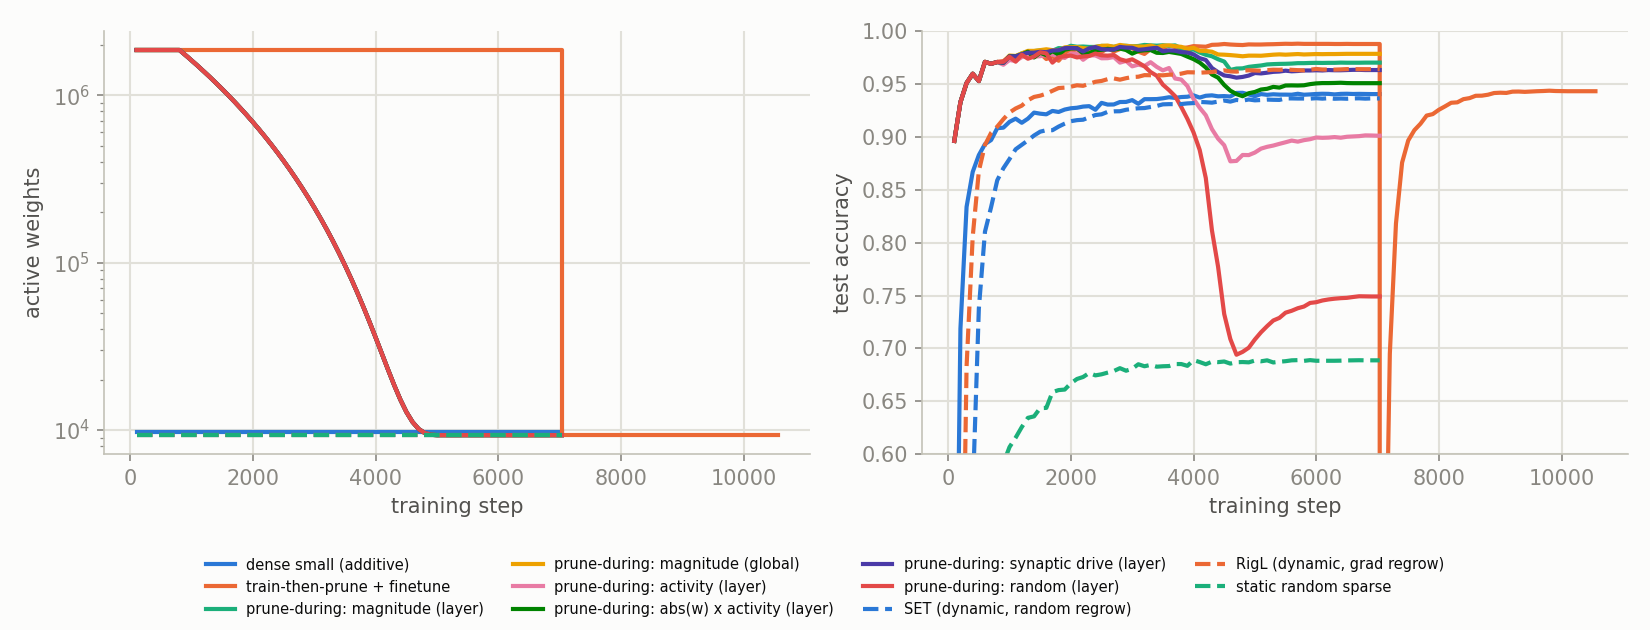
\includegraphics[width=\linewidth]{core_trajectory}
\caption{Connection count (left, log scale) and test accuracy (right) during training at 0.5\% density on MNIST (seed 0).
Prune-after (orange) trains dense, is pruned once at step 7035, collapses below 60\% and recovers to 94\% during fine-tuning;
the prune-during routes reach the same final count gradually; the global route (yellow) never falls below 97\% (lowest point
in any seed 97.3\%, run logs) and the per-layer route (green) ends at 97.0\%.}
\label{fig:traj}
\end{figure}

\paragraph{The benefit is in the gradual removal.} Figure~\ref{fig:traj} shows why prune-after loses at high sparsity: the
one-shot removal destroys the function and fine-tuning recovers only part of it. Gradual removal interleaved with learning
never leaves the high-accuracy region. The same picture holds on CIFAR-10 at 1\% (91.4\% before the pruning step, 10\%
after it, 80.5\% after fine-tuning; run logs). Sparsity itself is not the point: on MNIST the two routes that impose a random
pattern, a static random mask and random removal during training, are the worst at every budget below 10\% (72.7\% and
71.8\% at 0.5\%).

\paragraph{Connection counts versus FLOPs.} On the CNN, global magnitude pruning keeps convolutional weights, which are each
used at many positions, and removes fully connected ones, so the pruned network uses 2.4--3.5$\times$ the inference FLOPs of
the dense small network at the same connection count (Table~\ref{tab:cifar}). Constraining the per-layer allocation to ERK,
which on this CNN gives \emph{fewer} inference FLOPs than the dense small network, still leaves prune-during 4.2 points ahead
at 1\%, and 1.7--3.4 points ahead of RigL at the same FLOPs at 10\% and 3\% (5.4 at 1\% against the converged RigL seeds,
Table~\ref{tab:cifar}; Figure~\ref{fig:flops}). On ResNet-18 the ERK variant costs 2.3--2.5$\times$ the inference FLOPs of the dense small network,
so there the equal-FLOPs comparison holds only against RigL (Table~\ref{tab:resnet}). The gain is therefore real in both
currencies, but a paper that reports only connection counts would overstate it by a factor of 2.4--3.5 in compute.

\begin{figure}[t]
\centering
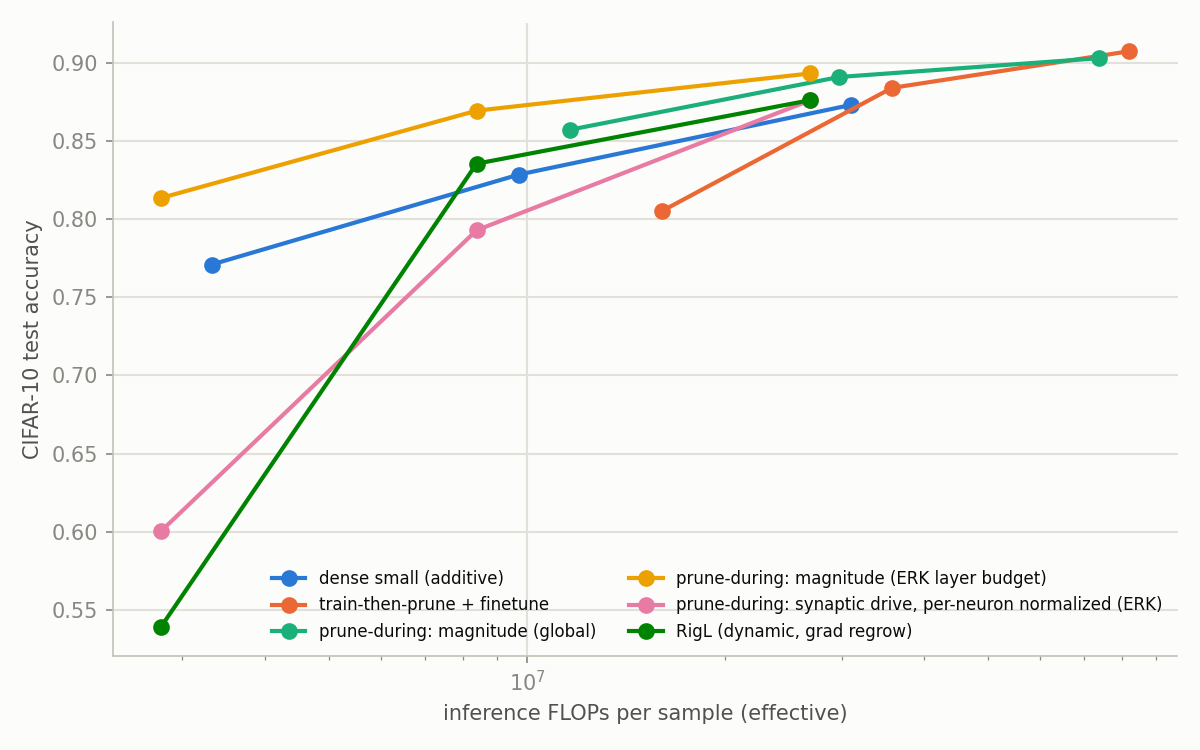
\includegraphics[width=0.8\linewidth]{core_inferflops_vs_acc_cifar}
\caption{CIFAR-10 accuracy against inference FLOPs; each point is one budget. At equal FLOPs, prune-during with the ERK
allocation (orange) dominates RigL (green) and the dense small network (blue). RigL at 1\% is plotted as its three-seed
mean (53.9\%), which includes the diverged seed.}
\label{fig:flops}
\end{figure}

\paragraph{Training cost, data efficiency, calibration.} Prune-during starts with the full network, so its cumulative training
FLOPs are 3$\times$ (10\%) to 50$\times$ (0.5\%) those of the dense small network on MNIST, 4.5--31$\times$ on CIFAR-10 and
8--59$\times$ on ResNet-18; prune-after costs a further 2.5--4$\times$. RigL costs about the same as the dense small network
on the MLP and CNN (as does SET, run on MNIST only) and 2.3--2.5$\times$ on ResNet-18. On the training-cost axis RigL is the most efficient of the
large-network routes; in accuracy it is second to prune-during only at the tightest budgets (0.5\% on MNIST and ResNet-18),
otherwise third behind prune-after, and at 1\% on CIFAR-10 it falls below the dense small network. Measured in samples rather
than FLOPs, the over-parameterised network learns fastest, but on MNIST it reaches 97\% after 87k samples, before pruning
begins, so this is a property of the dense start that every large-network route shares (against 133k--436k samples for the
dense small networks and 124k--445k for RigL). The comparison is informative where the target falls inside the pruning
phase: on ResNet-18 at 5\% prune-during reaches 85\% after 385k samples, when about a fifth of the weights remain, earlier
than the unpruned dense network (437k; prune-after is still dense at that point), RigL (524k) and the dense small network
(665k); at 0.5\% it needs 402k, against 437k, 908k (one RigL seed of three, the others never) and never. On MNIST the expected calibration error stays between 0.003 and 0.017 for the magnitude, additive, prune-after and
RigL routes at every budget and degrades for the local rules at the tightest budgets (drive 0.025, $|w|\times$activity
0.038, activity 0.100), for the static random mask (0.053) and for random removal (0.157); on the CNN and ResNet-18 all
routes lie between 0.008 and 0.038.

\paragraph{ResNet-18.} Table~\ref{tab:resnet} repeats the comparison with a CIFAR-style ResNet-18 (11.2M prunable
weights, 92.5\% dense; SGD, 20 epochs, three seeds) at 5\%, 2\% and 0.5\% of the weights. The winner is unchanged: at 0.5\%
(56k weights) prune-during reaches 89.0\% against 81.3\% for the dense small network, 83.6\% for prune-after and 84.9\% for
RigL, its largest lead over prune-after in any setting (5.3 points) and a lead over the additive baseline (7.7) close to the
CNN's (8.6); constrained to the ERK allocation it keeps 87.8\% at 40\% of the inference FLOPs of the global variant. The
order of the other routes does change with the model: on the CNN at 1\% prune-after beats dense small beats RigL, on
ResNet-18 at 0.5\% RigL beats prune-after beats dense small. At 5\% the three large-network routes lie within 0.3 points of
each other and within 0.5 points of the dense ceiling, so the budget, not the method, decides whether the route matters.

\begin{table}[t]
\centering\small
\caption{CIFAR-10 ResNet-18 (11.2M weights, 92.5\% dense): test accuracy (\%) and inference FLOPs per image at matched
budgets, three seeds. Per-layer criteria use the ERK allocation.}
\label{tab:resnet}
\begin{tabular}{lcccccc}
\toprule
 & \multicolumn{3}{c}{Accuracy} & \multicolumn{3}{c}{Inference FLOPs} \\
\cmidrule(lr){2-4}\cmidrule(lr){5-7}
Route (criterion) & 5\% & 2\% & 0.5\% & 5\% & 2\% & 0.5\% \\
\midrule
Dense small (additive)           & 88.7 & 86.5 & 81.3 & 5.6e7 & 2.3e7 & 6.1e6 \\
Prune-after + fine-tune          & \textbf{92.3} & 90.9 & 83.6 & 2.7e8 & 1.5e8 & 5.3e7 \\
Prune-during, magnitude (global) & 92.0 & \textbf{91.5} & \textbf{89.0} & 1.9e8 & 1.1e8 & 3.4e7 \\
Prune-during, magnitude (ERK)    & 92.0 & 91.3 & 87.8 & 1.4e8 & 5.7e7 & 1.4e7 \\
RigL (ERK)                       & 91.0 & 89.5 & 84.9 & 1.4e8 & 5.7e7 & 1.4e7 \\
\bottomrule
\end{tabular}
\end{table}

\paragraph{What to remove: local rules.} Removing connections by a Hebbian correlation trace beats random removal but falls
below the dense small network at every budget under 10\% (88.9\% against 94.1\% at 0.5\%), because $\mathbb{E}[y_i x_j]$
measures correlation through every path, not the contribution of synapse $ij$. Scoring synapses by their own drive repairs
most of the gap on the MLP: at 0.5\% the drive rule (96.0\%) beats the additive baseline, prune-after and SET and is 0.3
points behind RigL, with a criterion that uses no gradient information (training itself remains back-propagation). On the
CNN the unnormalised drive rule collapses within two epochs (run logs): channels that fire rarely lose all their inputs, die,
and the failure propagates downstream, a known hazard of activity-dependent pruning without homeostasis. Normalising each
neuron's drive by its mean removes the collapse but the rule still falls from parity with the dense baseline at 10\% to 17
points behind it at 1\%. A local criterion can stand in for the magnitude criterion on the MLP at a cost of 1.0 point at
0.5\% against the per-layer magnitude criterion (1.8 against the global one); on the convolutional network, in this form,
it cannot.

\paragraph{Transfer: pruning a pre-trained network during adaptation.} The over-parameterised starting point that
prune-during needs is, in practice, often inherited: pre-trained networks are published with their training cost already
paid, so the practical question is what gradual pruning does during adaptation.
We therefore took an ImageNet-pre-trained ResNet-18 (torchvision weights, 11.17M convolutional weights, fresh 10-way
classifier kept dense) and adapted it to CIFAR-10 for 10 epochs at $128\times128$ input while pruning its convolutions to 5\%,
2\% and 0.5\% with the same cubic schedule (SGD, lr 0.01, the from-scratch arms use lr 0.1 and the same architecture, schedule
and resolution). Table~\ref{tab:pretrained} compares gradual pruning during adaptation with one-shot magnitude pruning of the
same weights followed by fine-tuning, RigL started from a random ERK mask over the pre-trained weights, and the two from-scratch
routes. At 5\% and 2\% the pre-trained start is worth 5.3 and 3.5 points over pruning from scratch, gradual removal during
adaptation beats one-shot pruning of the same weights by 0.6--0.7 points, and RigL, which must discard the inherited
structure to start sparse, lands below pruning from scratch. The pre-trained prune-during arms reach 90\% after about 52k
samples (just over one epoch, when pruning has just begun and about 99\% of the weights remain, as does the dense
fine-tune), a level one-shot pruning needs
166k--402k samples for at 5\% and 2\% and does not reach at 0.5\%, and RigL never reaches in ten epochs; they are also
better calibrated (ECE 0.015--0.020 against 0.028--0.031 for prune-during from scratch). The inherited start does not save
adaptation compute: at 5\% gradual pruning costs 7.3e14 FLOPs from the pre-trained weights against 7.7e14 from scratch,
40\% of a dense fine-tune and 7$\times$ the dense small network. What it buys is accuracy; the early data efficiency is
that of the dense start, which gradual pruning keeps and one-shot pruning destroys. At 0.5\% the ordering reverses: pruning from scratch (83.8\%) beats one-shot pruning (81.7\%), which
beats gradual pruning of the pre-trained network (80.9\%). The pre-trained prune-during run peaks at 93.1\% in mid-schedule
and loses twelve points as the last 4.5\% of its connections go, with only three epochs left at the final density, whereas
one-shot pruning spends all ten there. An inherited structure pays off down to about 2\% of its connections; below that, a
magnitude profile tuned for another task is a liability, and the short adaptation window favours removing it at once.

\begin{table}[t]
\centering\small
\caption{ImageNet-pre-trained ResNet-18 adapted to CIFAR-10 ($128\times128$, 10 epochs) while being pruned: test accuracy
(\%) at matched convolutional budgets, two seeds, standard deviations $\le 0.4$. Adaptation FLOPs count the 10 epochs only;
the ImageNet pre-training is a sunk cost common to the pre-trained arms. The unpruned dense fine-tune reaches 95.9\% at
$1.8\times10^{15}$ FLOPs.}
\label{tab:pretrained}
\begin{tabular}{llcccc}
\toprule
Start & Route & 5\% & 2\% & 0.5\% & Adapt.\ FLOPs (5\%) \\
\midrule
pre-trained & prune-during, magnitude (global) & \textbf{93.7} & \textbf{91.0} & 80.9 & 7.3e14 \\
pre-trained & prune-during, magnitude (ERK)    & 93.4 & 89.7 & 78.8 & 8.1e14 \\
pre-trained & one-shot prune + fine-tune        & 93.1 & 90.3 & 81.7 & 3.0e14 \\
pre-trained & random ERK mask + RigL            & 86.9 & 83.6 & 76.8 & 2.7e14 \\
scratch     & prune-during, magnitude (global) & 88.4 & 87.5 & \textbf{83.8} & 7.7e14 \\
scratch     & dense small (additive)            & 84.8 & 82.4 & 76.5 & 1.1e14 \\
\bottomrule
\end{tabular}
\end{table}

\begin{figure}[t]
\centering
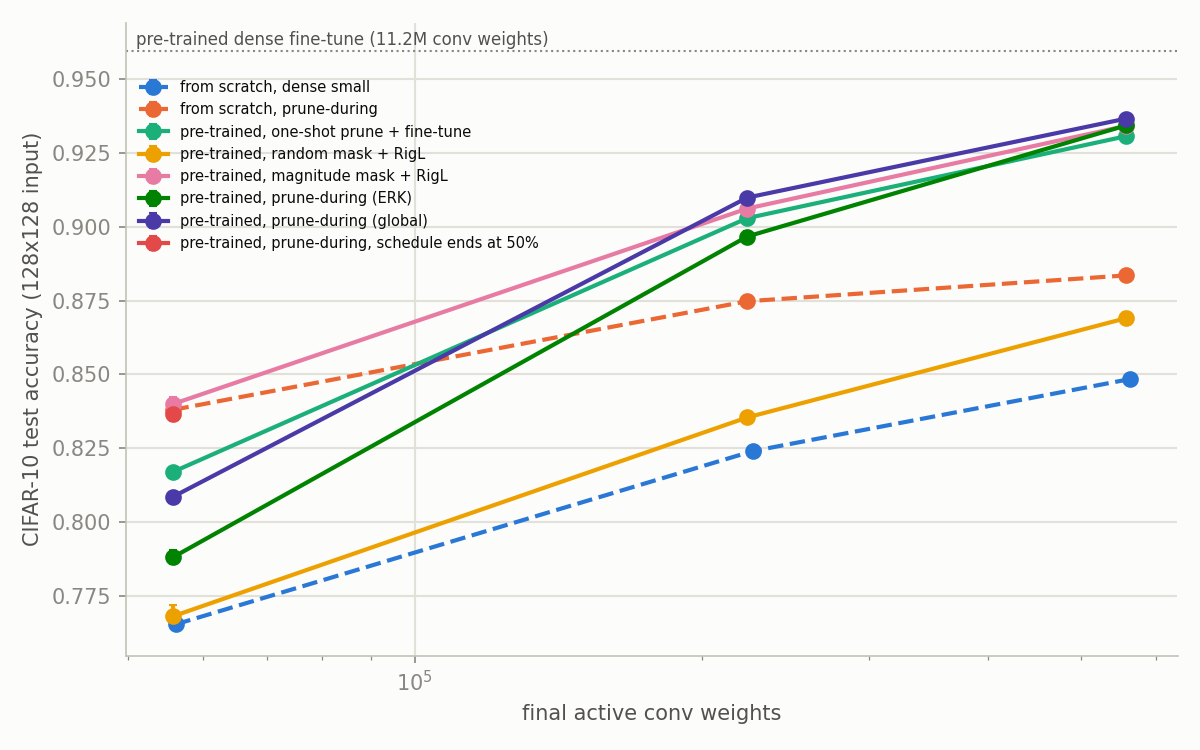
\includegraphics[width=0.75\linewidth]{core_pretrained_acc_vs_active}
\caption{Pre-trained ResNet-18 adapted to CIFAR-10 while pruned: accuracy against final active convolutional weights (two
seeds). Solid lines start from the ImageNet weights, dashed lines from scratch. The pre-trained advantage is largest at 5\% and
reverses at 0.5\%.}
\label{fig:pretrained}
\end{figure}

\section{Negative results from the same programme}
\label{sec:negative}

The programme that produced Section~\ref{sec:core} also implemented the other mechanisms of Table~\ref{tab:map}. Four
of them did not work as designed, and we report them because the failures are informative: sleep consolidation, thalamic
routing, predictive coding and per-input subnetworks. The local pruning criteria of Section~\ref{sec:core} are a variant of
the first mechanism and are not counted separately; the spiking network closes the section as a replication, not a
failure.

\begin{table}[t]
\centering\small
\caption{The mechanisms ported in this paper, their reductions, and what transferred.}
\label{tab:map}
\footnotesize
\begin{tabular}{@{}p{3.2cm}p{4.4cm}p{5.0cm}p{2.0cm}@{}}
\toprule
Brain mechanism & Our reduction & Outcome & Where \\
\midrule
gradual synaptic pruning during learning & prune-during at matched budgets & transfers (the principle; a schedule-level change) & Section~\ref{sec:core} \\
activity-dependent local pruning rules & Hebbian, drive and normalised-drive criteria & mixed: drive about a point behind per-layer magnitude pruning on the MLP, Hebbian eight points behind; the drive rules collapse on the CNN without homeostasis & Section~\ref{sec:core} \\
hippocampus--cortex sleep consolidation & fast/slow MLPs, replay, distillation, decay & does not transfer: matches class-balanced replay (beats plain replay by 1.2 points on Permuted MNIST at equal compute) & this section \\
thalamic routing & pre-decided skips; pre-routed attention & does not transfer (choice uninformative; little compute saved) & this section \\
predictive coding & skip by predicted change; predicted-residual substitution & does not transfer: selection no better than random, substitution no better than identity & this section \\
per-input subnetworks at inference (follow-up) & per-sample masks by a local rule & does not transfer & this section \\
spike-timing-dependent plasticity & Diehl--Cook network & mixed: known accuracy limit reproduced; self-sparsification observed & this section \\
\bottomrule
\end{tabular}
\end{table}

\paragraph{Sleep consolidation.} We trained a fast ``hippocampal'' MLP on the task stream and a slow ``cortical'' MLP only
during sleep phases at task boundaries, using the current task's data plus a 500-sample reservoir buffer, with distillation
from the fast network, global synaptic downscaling and magnitude or activity pruning as optional sleep ingredients
(Split MNIST class-incremental, Permuted MNIST, MLP 784--256--256--10, three seeds; Tables~\ref{tab:app-split} and
\ref{tab:app-permuted}). Distillation from the fast network lowered final average accuracy on Split MNIST from 85.0\% to
78.7\% and raised forgetting from 0.18 to 0.25, because the fast network, trained on the current task's classes alone under
the same single 10-way head, is biased to them; downscaling hurt in both settings (77.4\% and 82.7\%); magnitude pruning was neutral and
activity pruning cost 6.3 points on Permuted MNIST; and the scheme without distillation only matched plain experience replay
(85.0\% against 85.2\%) at three times the compute. A redesign with a $k$-winners-take-all sparse hippocampus, no distillation and
class-balanced replay improved to 87.0\%, but balanced sampling alone added to experience replay reaches 87.8\%, and the
hippocampal sparsity has no path to influence the cortex once distillation is removed. On Split MNIST the only effective
ingredient was the known one \citep{chrysakis2020}; on Permuted MNIST the scheme without distillation beats experience
replay by 1.2 points at the same compute (88.6\% against 87.4\%), and the sparse redesign beats balanced replay by 0.8
points at five times the compute (89.0\% against 88.3\%). This is a negative result for our simple implementation, not for the hippocampus--cortex
account: brain-inspired generative replay \citep{vandeven2020} and the hybrid CH-HNN \citep{shi2025} both succeed at
class-incremental learning, and what they have that we lacked is a hippocampus with generative capacity (internal
representations replayed through feedback connections) or a dual specific--generalised representation with episode inference, rather
than a second feed-forward network that can only speak to the cortex through distillation. Confidence-based agreement between the two networks, proposed as a metacognitive ``I do not
know'' signal, failed to detect unseen classes (AUROC 0.51), whereas plain softmax confidence reached 0.85. Varying how the
sleep phase decays weights, on the sparse redesign (Tables~\ref{tab:app-sleep-split} and \ref{tab:app-sleep-perm}), did not
change the picture: a one-shot 10\% downscaling at the task boundary, a gradual 10\% or 3\% decay spread over the sleep
phase and a continuous weight decay were within noise on Split MNIST (+0.1 to +0.5 points) and cost 0.3--4.0 points on
Permuted MNIST. Replacing global logit distillation by layer-local feature distillation, the form a processor--memory split
would favour, did not help: with a 256-unit fast network, local distillation costs 4.2 points against no distillation on
both benchmarks, less than global distillation on Split MNIST (6.2) and more on Permuted MNIST (1.6).

\paragraph{Predictive token skipping and pre-filtering.} With a low-rank predictor per block estimating how much each token
will change, skipping the tokens predicted to change least, uniformly over all blocks of a small ViT, was \emph{worse} than
skipping random tokens (MNIST, 30\% skip: 94.9\% against 96.7\%; even the oracle residual norm was worse than random), because
background tokens freeze consistently in every layer. Restricting skipping to the later half of the blocks recovers most of
the loss by itself: with the skipped tokens left unchanged and no fine-tuning, skipping 70\% of them in the late blocks costs
0.3 points on MNIST and 5.0 on CIFAR-10, against 1.5--3.3 and 8.9--15.4 points for skipping 30\% of them in every block at
slightly higher FLOPs (0.77 against 0.72 of the full model; Tables~\ref{tab:app-skip-mnist} and \ref{tab:app-skip-cifar}),
and a short
fine-tuning phase that ramps the skip ratio from 0 to 0.7 brings the CIFAR-10 cost to 1.0 point at 72\% of the FLOPs (ViT,
81.8\% baseline, one seed; Figure~\ref{fig:prefilter}). Replacing the skipped tokens by their predicted residual, the
predictive-coding ingredient, adds nothing over leaving them unchanged under the same fine-tuning: 97.9\% against 97.9\% on
MNIST (three seeds) and 80.8\% against 80.8\% on CIFAR-10 at 70\% skipping (one seed; within 0.7 points at every
non-zero ratio, with a 1.0-point gap at zero skipping that sets the single-seed noise floor;
Tables~\ref{tab:app-exp12-mnist} and \ref{tab:app-exp12-cifar}). A ``thalamic'' router that pre-decides all late-block skips from the representation at the block boundary performs identically
to per-block prediction and to random selection, also under cross-evaluation (three seeds on MNIST, one on CIFAR-10;
Tables~\ref{tab:app-exp12-mnist} and \ref{tab:app-exp12-cifar}). The choice of \emph{which} tokens to skip carries no
information at this scale, and neither does what replaces them; what matters is how many and in which layers.

\begin{figure}[t]
\centering
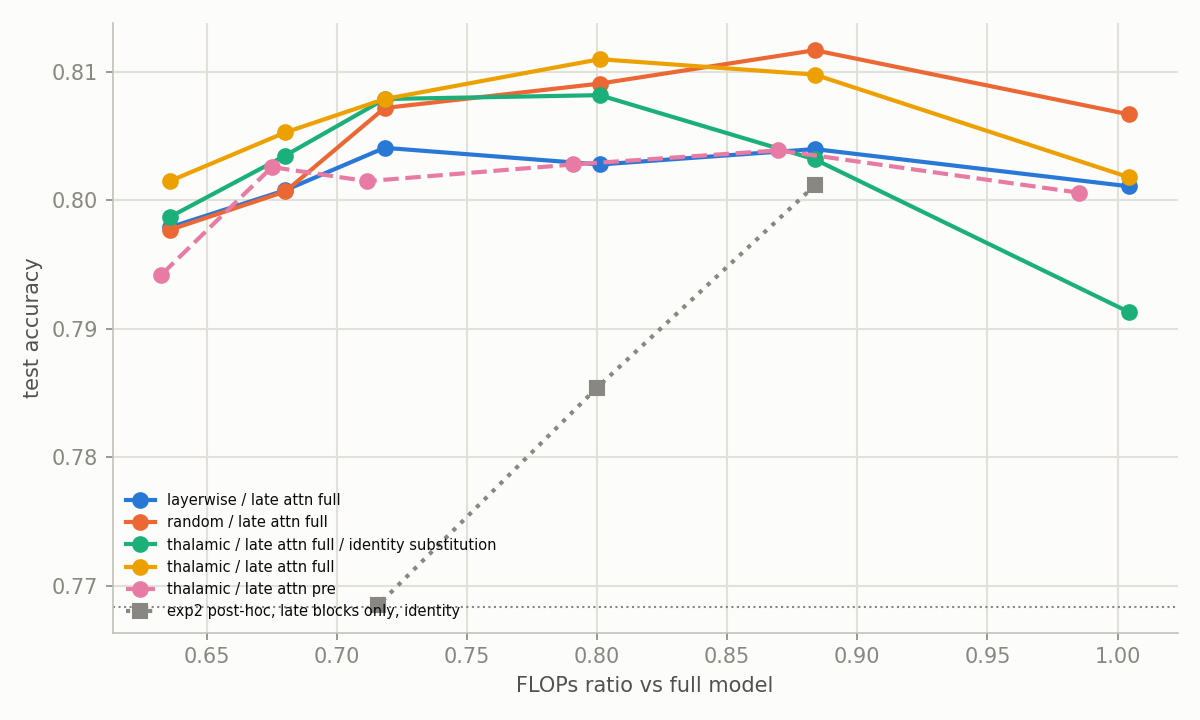
\includegraphics[width=0.8\linewidth]{exp12_cifar10}
\caption{CIFAR-10 ViT: accuracy against FLOPs when skipping tokens in the late blocks with predicted-residual substitution,
after fine-tuning with a ramped skip ratio (one seed). Thalamic pre-decision, per-block prediction, random selection and
identity substitution (no predicted residual) coincide; all lie far above post-hoc identity skipping without fine-tuning
(grey).}
\label{fig:prefilter}
\end{figure}

\paragraph{Pre-routed sparse attention.} Selecting the top-$k$ keys per query with an 8-dimensional router \emph{before} the
full attention computation keeps accuracy at $k=5$ of 50 keys on MNIST (98.1\% against 97.9\%, three seeds) and $k=17$ of 65
on CIFAR-10 (80.0\% against 79.4\%, one seed; Tables~\ref{tab:app-attn-mnist} and \ref{tab:app-attn-cifar}) and cuts
attention FLOPs by 68--77\%, but attention is only 5--6\% of the total cost at 50--65 tokens, so total FLOPs fall by only
3.6--4.7\%; post-hoc top-$k$ masking still computes the full score matrix and saves at most 2.7\%. Stacked on token skipping it saves a further
1\% of FLOPs for a 0.1--0.6 point loss. The mechanism is sound but irrelevant below several hundred tokens.

\paragraph{Input-dependent pruning at inference time.} If learning is pruning, should inference prune as well? We let
the ResNet-18 of Table~\ref{tab:resnet} select a different subnetwork for every input. For each output neuron, the connections
with the largest $|w_{ij}|\,\overline{|x_j|}$ (the weight times the mean magnitude of its input channel for that sample, a
per-sample form of the synaptic-drive rule without its post-synaptic term) are kept and the rest are masked for that sample
only, with the kept fraction following the same cubic schedule as prune-during so that every sample uses the budget (within
1\% at 20\% and 5\%; 14\% more at 0.5\%, where per-neuron rounding and the dense first layer dominate). Controls: the same per-sample
budget chosen at random, a channel-level $k$-WTA gate on each convolution's input (the only variant whose sparsity is structured
enough to save time on a GPU), and the static networks of Table~\ref{tab:resnet} plus a static mask with the same uniform
per-layer allocation that the dynamic rule is confined to. Table~\ref{tab:dynamic} gives the result. At 20\% the input-dependent
rule matches the fixed masks (91.8\% against 91.8--91.9\%). The penalty appears as the budget shrinks: at 5\% it reaches
89.8\% against 92.0\% for a fixed global mask and 91.1\% for a fixed mask with the same per-layer allocation, and at 0.5\%
77.7\% against 89.0\% and 83.1\%, so re-deciding the mask for every input costs 1.3 points at 5\% and 5.4 points at 0.5\%
even after allocation is controlled for; it beats the width-matched dense network at 20\% and 5\% (90.9\%, 88.7\%) and loses
to it at 0.5\% (81.3\%). In FLOPs the dynamic arm sits between the two fixed masks (at 0.5\%, 9.3e6 against 5.6e6 for the
uniform and 3.4e7 for the global mask). Random per-input selection collapses to 52.3\% at 5\% and 18.2\% at 0.5\%, and the channel-level
gate to 44.9\% and 34.0\% (73.4\% even at 20\%). The rule does form input-specific subnetworks: in the last stage, the masks
of two samples of the same class share 44\% of their connections at 5\% and those of different classes 27\% (random masks:
2.6\%; at 20\%, 61\% against 46\%), and across 200 test images the network touches 21\% of that stage's connections while
each image uses 5\%. The extra capacity is real and buys nothing. This is the mirror image of the token result: among tokens, which to drop did not matter; among
connections, which to keep is everything, and re-deciding it for every input is worse than deciding it once.

\begin{table}[t]
\centering\small\setlength{\tabcolsep}{4pt}
\caption{Input-dependent (per-sample) pruning of a CIFAR-10 ResNet-18 against fixed masks at the same per-sample budget.
Static rows from Table~\ref{tab:resnet} (three seeds; the 20\% column and the uniform-allocation control from
Table~\ref{tab:app-resnet}, two seeds); dynamic rows two seeds, with per-sample budgets within 1\% of the fixed masks at
20\% and 5\% and 14\% above them at 0.5\%. Jaccard: overlap of the last-stage masks of two test images of the same class / of different classes (200 images, 5\%
budget); a random mask gives 0.026.}
\label{tab:dynamic}
\begin{tabular}{lcccc}
\toprule
Mask & 20\% & 5\% & 0.5\% & Jaccard same / diff.\ class (5\%) \\
\midrule
fixed, prune-during, magnitude (global)               & \textbf{91.9} & \textbf{92.0} & \textbf{89.0} & -- \\
fixed, prune-during, magnitude (uniform per layer)    & 91.8 & 91.1 & 83.1 & -- \\
fixed, dense small (additive)                         & 90.9 & 88.7 & 81.3 & -- \\
per sample, connection-level, local rule              & 91.8 & 89.8 & 77.7 & 0.44 / 0.27 \\
per sample, connection-level, random                  & 76.1 & 52.3 & 18.2 & 0.03 / 0.03 \\
per sample, channel-level $k$-WTA gate                & 73.4 & 44.9 & 34.0 & 0.08 / 0.05 \\
\bottomrule
\end{tabular}
\end{table}

\paragraph{STDP sparsifies itself.} A 400-neuron spiking network in the style of \citet{diehl2015}, trained with
trace-based STDP, lateral inhibition and weight normalisation on one pass of MNIST, reaches 81.1$\pm$0.3\% (a
back-propagated MLP of the same width reaches 96.5\% on the same samples). The gap is the known limitation of unsupervised
STDP \citep{eshraghian2023,dong2023}; what we add is an observation about the weights. Without any explicit pruning, the
fraction of its input weights below 1\% of the maximum rises from 5.0\% to 57.7\% and the Gini coefficient of the weight
distribution from 0.33 to 0.77 during learning (run logs; the 100- and 1{,}600-neuron runs end at 54.9\% and 28.7\%,
Table~\ref{tab:app-stdp}). Learning under a local plasticity rule with normalisation is itself subtractive, which is the
biological reading of Section~\ref{sec:core}.

\section{Discussion and limitations}
\label{sec:discussion}

\paragraph{Scope of the claim.} The claim that survives is narrow and, we think, useful: at a tight final connection budget,
removing connections gradually while learning is better than learning small, better than removing them afterwards and better
than rewiring from a sparse start; the advantage grows with sparsity, and at loose budgets it shrinks to a tie with removing
them afterwards. The claim is about accuracy per connection. It is not a claim about training cost, where RigL wins, and on
convolutional networks it must be stated per FLOP as well as per connection. It is also not a claim that local rules suffice:
the best of them ends about a point behind per-layer magnitude pruning on the MLP, and the drive rules we ran on the CNN
fail there.

\paragraph{Training cost, and what an inherited start buys.} The 3--59$\times$ training-cost multiplier is the honest
weakness of prune-during trained from scratch: it buys accuracy with compute, and RigL buys most of the
accuracy for the price of the dense small network (2.3--2.5$\times$ on ResNet-18), trailing prune-during by 1.5--10 points
at the tightest budgets. Two observations qualify the weakness. First, training happens once and inference many times; at
equal inference FLOPs (the ERK-constrained variant) the extra training compute is amortised over deployment, so the trade-off
depends on how often the model is used. Second, the over-parameterised starting point is often inherited: pre-trained
networks are published with their training cost already paid. That does not make the adaptation cheap, since the schedule
still runs its dense phase (at 5\%, 7.3e14 FLOPs against 7.7e14 from scratch), but it changes what the compute buys. Pruning
pre-trained models is the classical setting of \citet{han2015} and
\citet{zhu2017}; what our comparison adds is that gradual removal \emph{during} adaptation should then dominate one-shot
pruning and, because RigL must discard the pre-trained structure to start sparse, dynamic sparse training as well. The
transfer experiment (Table~\ref{tab:pretrained}) confirms this at 5\% and 2\%: gradual removal during adaptation beats
one-shot pruning of the same weights, beats RigL on the pre-trained weights by seven points and keeps 5.3 and 3.5 points over
pruning from scratch, at 40\% of the FLOPs of a dense fine-tune. It refutes it at 0.5\%, where the inherited structure
becomes a liability and both one-shot pruning and training from scratch win: an inherited start pays off only while enough
of it survives. The developmental reading is the same: an organism inherits an over-connected
cortex it did not pay for and only pays for the pruning.

\paragraph{Scale.} Two small datasets; models from one to eleven million parameters. The ResNet-18 replication
(Table~\ref{tab:resnet}) shows that the winner and the growth of the margin with sparsity survive a five-fold increase in
model size, but ImageNet-scale data and models remain future work. The hazards we
found on the CNN (layer starvation under uniform allocation, channel death under activity pruning, divergence of RigL at
sub-1\% mid-layer densities) suggest that the extreme-sparsity regime will need care at scale.

\paragraph{What the negative results constrain.} A hippocampus that cannot communicate with the cortex except by distillation
will transfer its bias; a token-selection rule that freezes the same background tokens in every layer will lose to random
selection; an
attention-sparsity mechanism is only worth its router at long sequences; a network that re-selects its connections for every
input pays for the flexibility with accuracy. These are not arguments against the brain principles
but against the particular reductions we tried, and they are the kind of result that is rarely published and often re-discovered.

\paragraph{An observation about the failures.} We define a criterion and then apply it; it was formulated after the
experiments, so it is an organising observation rather than a prediction. We call a reduction a \emph{structure} when it
adds a component or a decision to the network (a second network, a router, a predictor that fills gaps, a per-sample mask);
a \emph{rule} when it replaces the pruning criterion or the learning rule by a local one, activity-based for the Hebbian and
drive criteria and STDP and activity-independent for the sleep decay variants; and a \emph{schedule} when it keeps the
magnitude criterion and changes only when and how much is removed. The principle of the abstract, learning as gradual pruning, is a schedule-level change in
these terms. Every structure failed. The rules were mixed: the drive criterion ends about a point behind per-layer magnitude
pruning on the MLP and collapses on the CNN, the decay variants were neutral or harmful, and STDP stays at its known
accuracy ceiling while sparsifying itself. Within the schedule level, the brain-derived gradual schedule beat the
conventional one-shot schedule (prune-after) at every tight budget when training from scratch, which is the paper's main
result (from a pre-trained start the order reverses at 0.5\%, Section~\ref{sec:core}); the sleep-phase
magnitude pruning of Section~\ref{sec:negative} was tested only inside the sleep structure, where it was neutral. One reading, offered as a hypothesis because it rests on a single positive case, is that a substantial
part of the brain's advantage rests on compute--memory unity, the hardware property by which every synapse computes, stores
and learns in place, and that a processor--memory architecture can imitate the structures only at a cost: a hippocampus
that can communicate only by distillation transfers its bias, a router must spend compute to save compute, a predictor must
be trained and evaluated for every token it stands in for, and a per-input subnetwork must be materialised as a per-sample
copy of the weights; the activity-based rules pay a smaller version of the same cost, tracking activity in buffers separate
from the weights they govern, and the decay variants add neither a module nor a buffer and simply did not help. Each failure also has a mundane explanation (bias transfer, a single shared head in class-incremental
learning, attention being 5--6\% of the cost, token selection carrying no information at this scale, a predicted residual
carrying no more than the token it replaces once only late layers are skipped, a mask that changes faster than the weights
can adapt to it), and the hippocampus--cortex structure has been made to work in software by giving the hippocampus
generative capacity or a hybrid dual representation \citep{vandeven2020,shi2025}. We did not test the hardware reading: in
our hands the gradual schedule transferred, the structures did not, and the rules were mixed.

\paragraph{Follow-up.} The natural next question links the main result to forgetting: whether networks sparsified by
prune-during interfere less across sequential tasks than dense networks of equal budget. This connects to PackNet-style
continual learning \citep{mallya2018,golkar2019} but tests the developmental claim directly.

\section{Conclusion}

Pruning during learning, with a plain global magnitude criterion and a gradual schedule, is the best route to a sparse network
at tight budgets on the three models we tried, ties with pruning afterwards at loose budgets, and its advantage comes from the
gradualness rather than from sparsity. Starting from a pre-trained network adds 3.5--5.3 points over pruning from scratch
down to about 2\% of the connections, without saving adaptation compute, and becomes a liability below that. The same programme's attempts at sleep consolidation, predictive skipping, thalamic routing (pre-decided skips and
pre-routed attention) and
input-dependent pruning did not add to known baselines, apart from a 1.2-point gain over plain replay on Permuted MNIST
at equal compute,
and we report them so that the next attempt can start from the right place.

\paragraph{Reproducibility.} Code, configurations, per-run logs and the full result tables are available at
\url{https://github.com/debtor114/subtractive-intelligence};
every number in this paper is produced by \texttt{scripts/analyze.py} from the stored run files.

\bibliographystyle{plainnat}
\bibliography{refs}

\appendix

\section{Hyper-parameters and implementation notes}

\paragraph{Masks.} Linear and convolutional layers carry a binary mask buffer; the forward pass uses $w \odot m$, masked
weights are re-zeroed after every optimiser step, and pruning selects an exact top-$k$ of the live weights by index so that
tied scores (common with activity traces) cannot inflate the count.

\paragraph{Schedules.} Prune-during: density $d(t)=d_f+(1-d_f)(1-t)^3$ for $t\in[0,1]$ spanning 10--70\% of training, pruning
every 100 steps, with a final pruning step at 70\% so that the target is met exactly. RigL/SET: drop fraction
$0.3\cdot\frac{1}{2}(1+\cos(\pi s/S))$ every 100 steps up to $S$ = 75\% of training. Prune-after: fine-tuning for half the
original epochs at lr 0.01 (CNN) or the original lr (MLP). RigL regrowth is skipped on steps whose mixed-precision gradients
are non-finite; without this guard one CIFAR-10 seed lost 93\% of its connections in the first 1{,}000 steps. With the guard
in place one CIFAR-10 seed at 1\% still diverged to chance (Table~\ref{tab:cifar}).

\paragraph{Dense small sizing.} MLP: hidden width $h$ solving $784h+h^2+10h=B$. CNN and ResNet: all widths scaled by a common
factor found by bisection on the prunable weight count.

\paragraph{Training.} MLP: Adam, lr $10^{-3}$, batch 128, one warm-up epoch then cosine, 15 epochs, no augmentation, full
training and test sets resident on the GPU. CNN: SGD with Nesterov momentum 0.9, lr 0.05, weight decay $5\times10^{-4}$ on
weights only, batch 128, mixed precision, 20 epochs, random crop (padding 4) and horizontal flip performed on the GPU.

\paragraph{Spiking network.} 784 Poisson inputs at 32\,Hz per unit intensity, 250\,ms per image, 1\,ms steps; 400 LIF
neurons with adaptive thresholds ($\theta^+=0.05$), 5\,ms refractory period, recurrent inhibition of 17.5\,mV; trace STDP with
$\eta_\mathrm{pre}=10^{-4}$, $\eta_\mathrm{post}=10^{-2}$; input weights normalised to a column sum of 78.4; batches of 32
images with summed updates. Labels are assigned to neurons by their class-wise mean response on 10k training images.

\section{Full result tables}
% generated by scripts/md_tables_to_tex.py -- lists every appendix table in order
Tables~\ref{tab:app-mnist}--\ref{tab:app-stdp} give every number behind the figures and tables of the main text, as mean $\pm$ standard deviation over seeds. FLOPs are analytic counts for one sample (inference) or accumulated over training at the actual density of each step. Five statements in the text rest on run logs rather than on these tables: the two-epoch collapse of the unnormalised drive rule on the CNN, the accuracy trajectory of prune-after on CIFAR-10 at its pruning step, the lowest point of the prune-during trajectory in Figure 1, the initial weight statistics of the spiking network, and its final Gini coefficient.

% generated by scripts/md_tables_to_tex.py from docs/report/tables/core_summary.md -- do not edit by hand
\begin{table}[p]
\centering
\footnotesize
\setlength{\tabcolsep}{3pt}
\resizebox{\textwidth}{!}{%
\begin{tabular}{llrrrrrrr}
\toprule
density & arm & seeds & active weights & test acc & ECE & infer FLOPs & cum. train FLOPs & samples to 97\% \\
\midrule
1 & dense big (no pruning) & 3 & 1,861,632 & 0.9871 $\pm$ 0.0003 & 0.009 $\pm$ 0.000 & $3.72\times10^{6}$ & $1.01\times10^{13}$ & 87336 $\pm$ 7781 \\
0.1 & dense small (additive) & 3 & 185,787 & 0.9836 $\pm$ 0.0003 & 0.009 $\pm$ 0.000 & $3.72\times10^{5}$ & $1.00\times10^{12}$ & 133096 $\pm$ 6988 \\
0.1 & prune-after: one-shot magnitude (global) + fine-tune & 3 & 186,163 & 0.9869 $\pm$ 0.0003 & 0.008 $\pm$ 0.000 & $3.72\times10^{5}$ & $1.06\times10^{13}$ & 87336 $\pm$ 7781 \\
0.1 & prune-after: gradual magnitude (global) during fine-tune & 3 & 186,163 & 0.9870 $\pm$ 0.0003 & 0.006 $\pm$ 0.000 & $3.72\times10^{5}$ & $1.18\times10^{13}$ & 87336 $\pm$ 7781 \\
0.1 & prune-during: magnitude (uniform per layer) & 3 & 186,164 & 0.9867 $\pm$ 0.0003 & 0.007 $\pm$ 0.000 & $3.72\times10^{5}$ & $3.33\times10^{12}$ & 87336 $\pm$ 7781 \\
0.1 & prune-during: magnitude (global) & 3 & 186,163 & 0.9867 $\pm$ 0.0002 & 0.008 $\pm$ 0.000 & $3.72\times10^{5}$ & $3.33\times10^{12}$ & 87336 $\pm$ 7781 \\
0.1 & prune-during: activity, Hebbian (uniform per layer) & 3 & 186,164 & 0.9819 $\pm$ 0.0007 & 0.004 $\pm$ 0.000 & $3.72\times10^{5}$ & $3.33\times10^{12}$ & 87336 $\pm$ 7781 \\
0.1 & prune-during: abs(w) $\times$ activity, Hebbian (uniform per layer) & 3 & 186,164 & 0.9857 $\pm$ 0.0004 & 0.006 $\pm$ 0.000 & $3.72\times10^{5}$ & $3.33\times10^{12}$ & 87336 $\pm$ 7781 \\
0.1 & prune-during: synaptic drive (uniform per layer) & 3 & 186,164 & 0.9853 $\pm$ 0.0004 & 0.007 $\pm$ 0.000 & $3.72\times10^{5}$ & $3.33\times10^{12}$ & 87336 $\pm$ 7781 \\
0.1 & prune-during: random (uniform per layer) & 3 & 186,164 & 0.9823 $\pm$ 0.0012 & 0.004 $\pm$ 0.000 & $3.72\times10^{5}$ & $3.33\times10^{12}$ & 87336 $\pm$ 7781 \\
0.1 & SET (dynamic sparse training, random regrowth) & 3 & 186,164 & 0.9838 $\pm$ 0.0004 & 0.010 $\pm$ 0.001 & $3.72\times10^{5}$ & $1.01\times10^{12}$ & 138766 $\pm$ 2328 \\
0.1 & RigL (dynamic sparse training, gradient regrowth) & 3 & 186,164 & 0.9853 $\pm$ 0.0011 & 0.008 $\pm$ 0.001 & $3.72\times10^{5}$ & $1.01\times10^{12}$ & 123519 $\pm$ 1928 \\
0.1 & static random sparse & 3 & 186,164 & 0.9818 $\pm$ 0.0002 & 0.006 $\pm$ 0.000 & $3.72\times10^{5}$ & $1.01\times10^{12}$ & 206096 $\pm$ 4555 \\
0.05 & dense small (additive) & 3 & 93,392 & 0.9801 $\pm$ 0.0003 & 0.009 $\pm$ 0.001 & $1.87\times10^{5}$ & $5.04\times10^{11}$ & 186445 $\pm$ 12401 \\
0.05 & prune-after: one-shot magnitude (global) + fine-tune & 3 & 93,082 & 0.9873 $\pm$ 0.0003 & 0.006 $\pm$ 0.000 & $1.86\times10^{5}$ & $1.03\times10^{13}$ & 87336 $\pm$ 7781 \\
0.05 & prune-after: gradual magnitude (global) during fine-tune & 3 & 93,082 & 0.9864 $\pm$ 0.0002 & 0.004 $\pm$ 0.000 & $1.86\times10^{5}$ & $1.16\times10^{13}$ & 87336 $\pm$ 7781 \\
0.05 & prune-during: magnitude (uniform per layer) & 3 & 93,082 & 0.9868 $\pm$ 0.0006 & 0.006 $\pm$ 0.001 & $1.86\times10^{5}$ & $2.96\times10^{12}$ & 87336 $\pm$ 7781 \\
0.05 & prune-during: magnitude (global) & 3 & 93,082 & 0.9872 $\pm$ 0.0003 & 0.006 $\pm$ 0.001 & $1.86\times10^{5}$ & $2.96\times10^{12}$ & 87336 $\pm$ 7781 \\
0.05 & prune-during: activity, Hebbian (uniform per layer) & 3 & 93,082 & 0.9787 $\pm$ 0.0001 & 0.005 $\pm$ 0.001 & $1.86\times10^{5}$ & $2.96\times10^{12}$ & 87336 $\pm$ 7781 \\
0.05 & prune-during: abs(w) $\times$ activity, Hebbian (uniform per layer) & 3 & 93,082 & 0.9842 $\pm$ 0.0004 & 0.004 $\pm$ 0.000 & $1.86\times10^{5}$ & $2.96\times10^{12}$ & 87336 $\pm$ 7781 \\
0.05 & prune-during: synaptic drive (uniform per layer) & 3 & 93,082 & 0.9850 $\pm$ 0.0003 & 0.005 $\pm$ 0.000 & $1.86\times10^{5}$ & $2.96\times10^{12}$ & 87336 $\pm$ 7781 \\
0.05 & prune-during: random (uniform per layer) & 3 & 93,082 & 0.9713 $\pm$ 0.0011 & 0.015 $\pm$ 0.000 & $1.86\times10^{5}$ & $2.96\times10^{12}$ & 87336 $\pm$ 7781 \\
0.05 & SET (dynamic sparse training, random regrowth) & 3 & 93,082 & 0.9819 $\pm$ 0.0009 & 0.006 $\pm$ 0.001 & $1.86\times10^{5}$ & $5.03\times10^{11}$ & 209140 $\pm$ 5774 \\
0.05 & RigL (dynamic sparse training, gradient regrowth) & 3 & 93,082 & 0.9822 $\pm$ 0.0004 & 0.008 $\pm$ 0.000 & $1.86\times10^{5}$ & $5.03\times10^{11}$ & 153687 $\pm$ 5905 \\
0.05 & static random sparse & 3 & 93,082 & 0.9754 $\pm$ 0.0003 & 0.004 $\pm$ 0.001 & $1.86\times10^{5}$ & $5.03\times10^{11}$ & 378278 $\pm$ 18120 \\
0.02 & dense small (additive) & 3 & 36,872 & 0.9730 $\pm$ 0.0010 & 0.006 $\pm$ 0.000 & $7.37\times10^{4}$ & $1.99\times10^{11}$ & 436301 $\pm$ 46700 \\
0.02 & prune-after: one-shot magnitude (global) + fine-tune & 3 & 37,233 & 0.9838 $\pm$ 0.0008 & 0.003 $\pm$ 0.001 & $7.45\times10^{4}$ & $1.02\times10^{13}$ & 87336 $\pm$ 7781 \\
0.02 & prune-after: gradual magnitude (global) during fine-tune & 3 & 37,233 & 0.9849 $\pm$ 0.0004 & 0.004 $\pm$ 0.000 & $7.45\times10^{4}$ & $1.15\times10^{13}$ & 87336 $\pm$ 7781 \\
0.02 & prune-during: magnitude (uniform per layer) & 3 & 37,233 & 0.9855 $\pm$ 0.0007 & 0.003 $\pm$ 0.000 & $7.45\times10^{4}$ & $2.73\times10^{12}$ & 87336 $\pm$ 7781 \\
0.02 & prune-during: magnitude (global) & 3 & 37,233 & 0.9865 $\pm$ 0.0002 & 0.003 $\pm$ 0.001 & $7.45\times10^{4}$ & $2.73\times10^{12}$ & 87336 $\pm$ 7781 \\
0.02 & prune-during: activity, Hebbian (uniform per layer) & 3 & 37,233 & 0.9655 $\pm$ 0.0009 & 0.020 $\pm$ 0.001 & $7.45\times10^{4}$ & $2.73\times10^{12}$ & 87336 $\pm$ 7781 \\
0.02 & prune-during: abs(w) $\times$ activity, Hebbian (uniform per layer) & 3 & 37,233 & 0.9805 $\pm$ 0.0004 & 0.005 $\pm$ 0.001 & $7.45\times10^{4}$ & $2.73\times10^{12}$ & 87336 $\pm$ 7781 \\
0.02 & prune-during: synaptic drive (uniform per layer) & 3 & 37,233 & 0.9822 $\pm$ 0.0003 & 0.004 $\pm$ 0.000 & $7.45\times10^{4}$ & $2.73\times10^{12}$ & 87336 $\pm$ 7781 \\
0.02 & prune-during: random (uniform per layer) & 3 & 37,233 & 0.9339 $\pm$ 0.0015 & 0.034 $\pm$ 0.002 & $7.45\times10^{4}$ & $2.73\times10^{12}$ & 87336 $\pm$ 7781 \\
0.02 & SET (dynamic sparse training, random regrowth) & 3 & 37,233 & 0.9743 $\pm$ 0.0006 & 0.005 $\pm$ 0.000 & $7.45\times10^{4}$ & $2.01\times10^{11}$ & 467683 $\pm$ 20709 \\
0.02 & RigL (dynamic sparse training, gradient regrowth) & 3 & 37,233 & 0.9785 $\pm$ 0.0004 & 0.005 $\pm$ 0.001 & $7.45\times10^{4}$ & $2.01\times10^{11}$ & 245749 $\pm$ 12815 \\
0.02 & static random sparse & 3 & 37,233 & 0.9590 $\pm$ 0.0013 & 0.009 $\pm$ 0.001 & $7.45\times10^{4}$ & $2.01\times10^{11}$ & - \\
0.01 & dense small (additive) & 3 & 18,791 & 0.9630 $\pm$ 0.0012 & 0.004 $\pm$ 0.001 & $3.76\times10^{4}$ & $1.01\times10^{11}$ & - \\
0.01 & prune-after: one-shot magnitude (global) + fine-tune & 3 & 18,616 & 0.9752 $\pm$ 0.0020 & 0.006 $\pm$ 0.000 & $3.72\times10^{4}$ & $1.01\times10^{13}$ & 87336 $\pm$ 7781 \\
0.01 & prune-after: gradual magnitude (global) during fine-tune & 3 & 18,616 & 0.9794 $\pm$ 0.0006 & 0.009 $\pm$ 0.000 & $3.72\times10^{4}$ & $1.14\times10^{13}$ & 87336 $\pm$ 7781 \\
0.01 & prune-during: magnitude (uniform per layer) & 3 & 18,616 & 0.9823 $\pm$ 0.0001 & 0.007 $\pm$ 0.000 & $3.72\times10^{4}$ & $2.66\times10^{12}$ & 87336 $\pm$ 7781 \\
0.01 & prune-during: magnitude (global) & 3 & 18,616 & 0.9844 $\pm$ 0.0003 & 0.004 $\pm$ 0.000 & $3.72\times10^{4}$ & $2.66\times10^{12}$ & 87336 $\pm$ 7781 \\
0.01 & prune-during: activity, Hebbian (uniform per layer) & 3 & 18,616 & 0.9366 $\pm$ 0.0015 & 0.037 $\pm$ 0.001 & $3.72\times10^{4}$ & $2.66\times10^{12}$ & 87336 $\pm$ 7781 \\
0.01 & prune-during: abs(w) $\times$ activity, Hebbian (uniform per layer) & 3 & 18,616 & 0.9725 $\pm$ 0.0008 & 0.012 $\pm$ 0.001 & $3.72\times10^{4}$ & $2.66\times10^{12}$ & 87336 $\pm$ 7781 \\
0.01 & prune-during: synaptic drive (uniform per layer) & 3 & 18,616 & 0.9756 $\pm$ 0.0010 & 0.012 $\pm$ 0.000 & $3.72\times10^{4}$ & $2.66\times10^{12}$ & 87336 $\pm$ 7781 \\
0.01 & prune-during: random (uniform per layer) & 3 & 18,616 & 0.8913 $\pm$ 0.0060 & 0.071 $\pm$ 0.003 & $3.72\times10^{4}$ & $2.66\times10^{12}$ & 87336 $\pm$ 7781 \\
0.01 & SET (dynamic sparse training, random regrowth) & 3 & 18,616 & 0.9603 $\pm$ 0.0010 & 0.008 $\pm$ 0.001 & $3.72\times10^{4}$ & $1.01\times10^{11}$ & - \\
0.01 & RigL (dynamic sparse training, gradient regrowth) & 3 & 18,616 & 0.9741 $\pm$ 0.0016 & 0.004 $\pm$ 0.001 & $3.72\times10^{4}$ & $1.01\times10^{11}$ & 444658 $\pm$ 67026 \\
0.01 & RigL, 3x training length & 3 & 18,616 & 0.9772 $\pm$ 0.0008 & 0.013 $\pm$ 0.001 & $3.72\times10^{4}$ & $3.02\times10^{11}$ & 445880 $\pm$ 52617 \\
0.01 & static random sparse & 3 & 18,616 & 0.9259 $\pm$ 0.0034 & 0.015 $\pm$ 0.001 & $3.72\times10^{4}$ & $1.01\times10^{11}$ & - \\
0.005 & dense small (additive) & 3 & 9,672 & 0.9407 $\pm$ 0.0010 & 0.009 $\pm$ 0.001 & $1.93\times10^{4}$ & $5.22\times10^{10}$ & - \\
0.005 & prune-after: one-shot magnitude (global) + fine-tune & 3 & 9,308 & 0.9451 $\pm$ 0.0060 & 0.017 $\pm$ 0.006 & $1.86\times10^{4}$ & $1.01\times10^{13}$ & 87336 $\pm$ 7781 \\
0.005 & prune-after: gradual magnitude (global) during fine-tune & 3 & 9,308 & 0.9692 $\pm$ 0.0012 & 0.020 $\pm$ 0.001 & $1.86\times10^{4}$ & $1.14\times10^{13}$ & 87336 $\pm$ 7781 \\
0.005 & prune-during: magnitude (uniform per layer) & 3 & 9,308 & 0.9704 $\pm$ 0.0005 & 0.015 $\pm$ 0.001 & $1.86\times10^{4}$ & $2.62\times10^{12}$ & 87336 $\pm$ 7781 \\
0.005 & prune-during: magnitude (global) & 3 & 9,308 & 0.9781 $\pm$ 0.0002 & 0.006 $\pm$ 0.000 & $1.86\times10^{4}$ & $2.62\times10^{12}$ & 87336 $\pm$ 7781 \\
0.005 & prune-during: activity, Hebbian (uniform per layer) & 3 & 9,322 & 0.8885 $\pm$ 0.0109 & 0.100 $\pm$ 0.037 & $1.86\times10^{4}$ & $2.62\times10^{12}$ & 87336 $\pm$ 7781 \\
0.005 & prune-during: abs(w) $\times$ activity, Hebbian (uniform per layer) & 3 & 9,308 & 0.9522 $\pm$ 0.0013 & 0.038 $\pm$ 0.016 & $1.86\times10^{4}$ & $2.62\times10^{12}$ & 87336 $\pm$ 7781 \\
0.005 & prune-during: synaptic drive (uniform per layer) & 3 & 9,308 & 0.9603 $\pm$ 0.0020 & 0.025 $\pm$ 0.000 & $1.86\times10^{4}$ & $2.62\times10^{12}$ & 87336 $\pm$ 7781 \\
0.005 & prune-during: random (uniform per layer) & 3 & 9,308 & 0.7184 $\pm$ 0.0230 & 0.157 $\pm$ 0.017 & $1.86\times10^{4}$ & $2.62\times10^{12}$ & 87336 $\pm$ 7781 \\
0.005 & SET (dynamic sparse training, random regrowth) & 3 & 9,308 & 0.9365 $\pm$ 0.0011 & 0.012 $\pm$ 0.001 & $1.86\times10^{4}$ & $5.03\times10^{10}$ & - \\
0.005 & RigL (dynamic sparse training, gradient regrowth) & 3 & 9,308 & 0.9631 $\pm$ 0.0027 & 0.005 $\pm$ 0.001 & $1.86\times10^{4}$ & $5.03\times10^{10}$ & - \\
0.005 & RigL, 3x training length & 3 & 9,308 & 0.9746 $\pm$ 0.0010 & 0.008 $\pm$ 0.001 & $1.86\times10^{4}$ & $1.51\times10^{11}$ & 844057 $\pm$ 92020 \\
0.005 & static random sparse & 3 & 9,308 & 0.7271 $\pm$ 0.0271 & 0.053 $\pm$ 0.012 & $1.86\times10^{4}$ & $5.03\times10^{10}$ & - \\
\bottomrule
\end{tabular}}
\caption{MNIST MLP (784-1024-1024-10, 1.86M weights), all arms and budgets, 3 seeds. Density is the final active fraction of the over-parameterised network; dense small is a width-matched network at the same budget. Training FLOPs count three forward passes per step at the actual density of that step.}
\label{tab:app-mnist}
\end{table}

% generated by scripts/md_tables_to_tex.py from docs/report/tables/core_summary_cifar.md -- do not edit by hand
\begin{table}[p]
\centering
\footnotesize
\setlength{\tabcolsep}{3pt}
\resizebox{\textwidth}{!}{%
\begin{tabular}{llrrrrrrr}
\toprule
density & arm & seeds & active weights & test acc & ECE & infer FLOPs & cum. train FLOPs & samples to 85\% \\
\midrule
1 & dense big (no pruning) & 3 & 2,195,648 & 0.9133 $\pm$ 0.0010 & 0.031 $\pm$ 0.001 & $3.08\times10^{8}$ & $9.23\times10^{14}$ & 411367 $\pm$ 15611 \\
0.1 & dense small (additive) & 3 & 219,735 & 0.8729 $\pm$ 0.0007 & 0.029 $\pm$ 0.001 & $3.10\times10^{7}$ & $9.31\times10^{13}$ & 632089 $\pm$ 19636 \\
0.1 & dense small, shallow and wide (additive) & 3 & 219,918 & 0.8685 $\pm$ 0.0026 & 0.025 $\pm$ 0.002 & $8.09\times10^{7}$ & $2.43\times10^{14}$ & 676291 $\pm$ 26535 \\
0.1 & prune-after: one-shot magnitude (global) + fine-tune & 3 & 219,565 & 0.9072 $\pm$ 0.0014 & 0.036 $\pm$ 0.001 & $8.19\times10^{7}$ & $1.05\times10^{15}$ & 411367 $\pm$ 15611 \\
0.1 & prune-after: gradual magnitude (global) during fine-tune & 3 & 219,565 & 0.9051 $\pm$ 0.0023 & 0.036 $\pm$ 0.002 & $8.05\times10^{7}$ & $1.15\times10^{15}$ & 440414 $\pm$ 23340 \\
0.1 & prune-during: magnitude (global) & 3 & 219,565 & 0.9028 $\pm$ 0.0029 & 0.033 $\pm$ 0.001 & $7.37\times10^{7}$ & $4.19\times10^{14}$ & 387708 $\pm$ 26819 \\
0.1 & prune-during: magnitude (ERK per layer) & 3 & 219,565 & 0.8930 $\pm$ 0.0004 & 0.030 $\pm$ 0.001 & $2.69\times10^{7}$ & $2.80\times10^{14}$ & 374564 $\pm$ 22672 \\
0.1 & prune-during: synaptic drive, per-neuron normalised (ERK per layer) & 3 & 219,565 & 0.8759 $\pm$ 0.0033 & 0.026 $\pm$ 0.003 & $2.69\times10^{7}$ & $2.80\times10^{14}$ & 633096 $\pm$ 45722 \\
0.1 & RigL (dynamic sparse training, gradient regrowth) & 3 & 219,565 & 0.8759 $\pm$ 0.0005 & 0.026 $\pm$ 0.002 & $2.69\times10^{7}$ & $8.07\times10^{13}$ & 625325 $\pm$ 28326 \\
0.03 & dense small (additive) & 3 & 67,905 & 0.8284 $\pm$ 0.0010 & 0.024 $\pm$ 0.001 & $9.72\times10^{6}$ & $2.92\times10^{13}$ & - \\
0.03 & dense small, shallow and wide (additive) & 3 & 68,264 & 0.8391 $\pm$ 0.0008 & 0.019 $\pm$ 0.001 & $2.57\times10^{7}$ & $7.72\times10^{13}$ & - \\
0.03 & prune-after: one-shot magnitude (global) + fine-tune & 3 & 65,869 & 0.8838 $\pm$ 0.0022 & 0.026 $\pm$ 0.001 & $3.58\times10^{7}$ & $9.77\times10^{14}$ & 411367 $\pm$ 15611 \\
0.03 & prune-after: gradual magnitude (global) during fine-tune & 3 & 65,869 & 0.8797 $\pm$ 0.0011 & 0.022 $\pm$ 0.001 & $3.42\times10^{7}$ & $1.11\times10^{15}$ & 440414 $\pm$ 23340 \\
0.03 & prune-during: magnitude (global) & 3 & 65,869 & 0.8908 $\pm$ 0.0017 & 0.028 $\pm$ 0.002 & $2.98\times10^{7}$ & $3.40\times10^{14}$ & 391024 $\pm$ 6160 \\
0.03 & prune-during: magnitude (ERK per layer) & 3 & 65,870 & 0.8692 $\pm$ 0.0026 & 0.023 $\pm$ 0.003 & $8.38\times10^{6}$ & $2.39\times10^{14}$ & 495322 $\pm$ 145564 \\
0.03 & prune-during: synaptic drive, per-neuron normalised (ERK per layer) & 3 & 65,870 & 0.7928 $\pm$ 0.0048 & 0.020 $\pm$ 0.003 & $8.38\times10^{6}$ & $2.39\times10^{14}$ & - \\
0.03 & RigL (dynamic sparse training, gradient regrowth) & 3 & 65,870 & 0.8353 $\pm$ 0.0019 & 0.018 $\pm$ 0.001 & $8.38\times10^{6}$ & $2.52\times10^{13}$ & - \\
0.03 & RigL, 3x training length & 3 & 65,870 & 0.8702 $\pm$ 0.0022 & 0.025 $\pm$ 0.001 & $8.38\times10^{6}$ & $7.55\times10^{13}$ & 1909949 $\pm$ 39835 \\
0.01 & dense small (additive) & 3 & 22,911 & 0.7709 $\pm$ 0.0036 & 0.020 $\pm$ 0.004 & $3.32\times10^{6}$ & $9.97\times10^{12}$ & - \\
0.01 & dense small, shallow and wide (additive) & 3 & 22,074 & 0.7836 $\pm$ 0.0026 & 0.016 $\pm$ 0.002 & $8.53\times10^{6}$ & $2.56\times10^{13}$ & - \\
0.01 & prune-after: one-shot magnitude (global) + fine-tune & 3 & 21,956 & 0.8051 $\pm$ 0.0010 & 0.015 $\pm$ 0.003 & $1.60\times10^{7}$ & $9.47\times10^{14}$ & 411367 $\pm$ 15611 \\
0.01 & prune-after: gradual magnitude (global) during fine-tune & 3 & 21,956 & 0.8192 $\pm$ 0.0021 & 0.012 $\pm$ 0.002 & $1.47\times10^{7}$ & $1.09\times10^{15}$ & 440414 $\pm$ 23340 \\
0.01 & prune-during: magnitude (global) & 3 & 21,956 & 0.8570 $\pm$ 0.0020 & 0.023 $\pm$ 0.001 & $1.16\times10^{7}$ & $3.09\times10^{14}$ & 390029 $\pm$ 6850 \\
0.01 & prune-during: magnitude (ERK per layer) & 3 & 21,957 & 0.8134 $\pm$ 0.0007 & 0.015 $\pm$ 0.001 & $2.78\times10^{6}$ & $2.27\times10^{14}$ & - \\
0.01 & prune-during: synaptic drive, per-neuron normalised (ERK per layer) & 3 & 21,957 & 0.6004 $\pm$ 0.0141 & 0.013 $\pm$ 0.006 & $2.78\times10^{6}$ & $2.27\times10^{14}$ & - \\
0.01 & RigL (dynamic sparse training, gradient regrowth) & 3 & 21,957 & 0.5392 $\pm$ 0.3110 & 0.008 $\pm$ 0.006 & $2.78\times10^{6}$ & $8.35\times10^{12}$ & - \\
0.01 & RigL, 3x training length & 3 & 21,957 & 0.5666 $\pm$ 0.3299 & 0.010 $\pm$ 0.007 & $2.78\times10^{6}$ & $2.50\times10^{13}$ & - \\
\bottomrule
\end{tabular}}
\caption{CIFAR-10 CNN (2.2M weights), all arms and budgets, 3 seeds. Columns as in Table~\ref{tab:app-mnist}; the data-efficiency column is the number of training samples until 85\% test accuracy.}
\label{tab:app-cifar}
\end{table}

% generated by scripts/md_tables_to_tex.py from docs/report/tables/core_summary_resnet.md -- do not edit by hand
\begin{table}[p]
\centering
\footnotesize
\setlength{\tabcolsep}{3pt}
\resizebox{\textwidth}{!}{%
\begin{tabular}{llrrrrrrr}
\toprule
density & arm & seeds & active weights & test acc & ECE & infer FLOPs & cum. train FLOPs & samples to 85\% \\
\midrule
1 & dense big (no pruning) & 3 & 11,164,352 & 0.9248 $\pm$ 0.0026 & 0.035 $\pm$ 0.001 & $1.11\times10^{9}$ & $3.33\times10^{15}$ & 436855 $\pm$ 29455 \\
0.2 & dense small (additive) & 2 & 2,239,484 & 0.9093 $\pm$ 0.0000 & 0.035 $\pm$ 0.002 & $2.25\times10^{8}$ & $6.74\times10^{14}$ & 514366 $\pm$ 32163 \\
0.2 & prune-during: magnitude (layer) & 2 & 2,232,871 & 0.9179 $\pm$ 0.0009 & 0.038 $\pm$ 0.000 & $2.22\times10^{8}$ & $1.35\times10^{15}$ & 382401 $\pm$ 5235 \\
0.2 & prune-during: magnitude (global) & 2 & 2,232,870 & 0.9189 $\pm$ 0.0013 & 0.038 $\pm$ 0.000 & $3.45\times10^{8}$ & $1.65\times10^{15}$ & 377044 $\pm$ 750 \\
0.05 & dense small (additive) & 3 & 562,229 & 0.8866 $\pm$ 0.0018 & 0.030 $\pm$ 0.002 & $5.58\times10^{7}$ & $1.67\times10^{14}$ & 665417 $\pm$ 15510 \\
0.05 & train-then-prune + finetune & 3 & 558,218 & 0.9227 $\pm$ 0.0006 & 0.035 $\pm$ 0.001 & $2.71\times10^{8}$ & $3.74\times10^{15}$ & 434143 $\pm$ 30338 \\
0.05 & prune-during: magnitude (layer) & 2 & 558,217 & 0.9108 $\pm$ 0.0002 & 0.037 $\pm$ 0.001 & $5.55\times10^{7}$ & $9.79\times10^{14}$ & 387334 $\pm$ 8668 \\
0.05 & prune-during: magnitude (global) & 3 & 558,218 & 0.9196 $\pm$ 0.0023 & 0.034 $\pm$ 0.001 & $1.85\times10^{8}$ & $1.33\times10^{15}$ & 384521 $\pm$ 15853 \\
0.05 & prune-during: magnitude (ERK layer budget) & 3 & 558,213 & 0.9203 $\pm$ 0.0009 & 0.034 $\pm$ 0.001 & $1.39\times10^{8}$ & $1.43\times10^{15}$ & 399622 $\pm$ 18599 \\
0.05 & RigL (dynamic, grad regrow) & 3 & 558,213 & 0.9097 $\pm$ 0.0016 & 0.034 $\pm$ 0.001 & $1.39\times10^{8}$ & $4.17\times10^{14}$ & 524129 $\pm$ 20642 \\
0.02 & dense small (additive) & 3 & 225,892 & 0.8647 $\pm$ 0.0030 & 0.026 $\pm$ 0.000 & $2.25\times10^{7}$ & $6.76\times10^{13}$ & 801128 $\pm$ 18275 \\
0.02 & train-then-prune + finetune & 3 & 223,287 & 0.9094 $\pm$ 0.0018 & 0.027 $\pm$ 0.002 & $1.49\times10^{8}$ & $3.56\times10^{15}$ & 434143 $\pm$ 30338 \\
0.02 & prune-during: magnitude (global) & 3 & 223,287 & 0.9146 $\pm$ 0.0015 & 0.034 $\pm$ 0.002 & $1.07\times10^{8}$ & $1.20\times10^{15}$ & 388422 $\pm$ 24257 \\
0.02 & prune-during: magnitude (ERK layer budget) & 3 & 223,288 & 0.9125 $\pm$ 0.0012 & 0.032 $\pm$ 0.001 & $5.71\times10^{7}$ & $1.26\times10^{15}$ & 394149 $\pm$ 11727 \\
0.02 & RigL (dynamic, grad regrow) & 3 & 223,288 & 0.8950 $\pm$ 0.0018 & 0.030 $\pm$ 0.003 & $5.71\times10^{7}$ & $1.71\times10^{14}$ & 597590 $\pm$ 17418 \\
0.005 & dense small (additive) & 3 & 55,872 & 0.8131 $\pm$ 0.0026 & 0.021 $\pm$ 0.001 & $6.12\times10^{6}$ & $1.84\times10^{13}$ & - \\
0.005 & train-then-prune + finetune & 3 & 55,822 & 0.8364 $\pm$ 0.0015 & 0.016 $\pm$ 0.001 & $5.27\times10^{7}$ & $3.41\times10^{15}$ & 445811 $\pm$ 28637 \\
0.005 & prune-during: magnitude (layer) & 2 & 55,819 & 0.8311 $\pm$ 0.0006 & 0.022 $\pm$ 0.001 & $5.55\times10^{6}$ & $8.67\times10^{14}$ & 392455 $\pm$ 2533 \\
0.005 & prune-during: magnitude (global) & 3 & 55,822 & 0.8896 $\pm$ 0.0003 & 0.027 $\pm$ 0.001 & $3.40\times10^{7}$ & $1.09\times10^{15}$ & 401879 $\pm$ 17074 \\
0.005 & prune-during: magnitude (ERK layer budget) & 3 & 55,820 & 0.8783 $\pm$ 0.0022 & 0.024 $\pm$ 0.001 & $1.38\times10^{7}$ & $1.18\times10^{15}$ & 391071 $\pm$ 8159 \\
0.005 & RigL (dynamic, grad regrow) & 3 & 55,820 & 0.8486 $\pm$ 0.0030 & 0.026 $\pm$ 0.001 & $1.38\times10^{7}$ & $4.15\times10^{13}$ & 907936 \\
\bottomrule
\end{tabular}}
\caption{CIFAR-10 ResNet-18 (11.2M weights), all arms and budgets. Columns as in Table~\ref{tab:app-mnist}; samples to 85\% test accuracy.}
\label{tab:app-resnet}
\end{table}

% generated by scripts/md_tables_to_tex.py from docs/report/tables/core_pretrained_summary.md -- do not edit by hand
\begin{sidewaystable}[p]
\centering
\footnotesize
\setlength{\tabcolsep}{3pt}
\resizebox{\textwidth}{!}{%
\begin{tabular}{llrrrrrrrrr}
\toprule
density & arm & seeds & active conv weights & init acc & final acc & best acc & ECE & infer FLOPs & adaptation train FLOPs & samples to 90\% \\
\midrule
1 & pre-trained, dense fine-tune (no pruning) & 2 & 11,166,912 & 0.1085 $\pm$ 0.0170 & 0.9593 $\pm$ 0.0000 & 0.9598 $\pm$ 0.0000 & 0.018 $\pm$ 0.001 & $1.18\times10^{9}$ & $1.78\times10^{15}$ & 52515 $\pm$ 1566 \\
0.05 & from scratch, dense small (width-scaled) & 2 & 562,759 & 0.1000 $\pm$ 0.0000 & 0.8484 $\pm$ 0.0004 & 0.8486 $\pm$ 0.0006 & 0.022 $\pm$ 0.001 & $7.19\times10^{7}$ & $1.08\times10^{14}$ & - \\
0.05 & from scratch, prune-during (global magnitude) & 2 & 558,346 & 0.1000 $\pm$ 0.0000 & 0.8835 $\pm$ 0.0007 & 0.8838 $\pm$ 0.0010 & 0.031 $\pm$ 0.001 & $2.40\times10^{8}$ & $7.72\times10^{14}$ & - \\
0.05 & pre-trained, one-shot prune then fine-tune & 2 & 558,346 & 0.1000 $\pm$ 0.0000 & 0.9306 $\pm$ 0.0012 & 0.9316 $\pm$ 0.0007 & 0.020 $\pm$ 0.001 & $2.01\times10^{8}$ & $3.02\times10^{14}$ & 165526 $\pm$ 4694 \\
0.05 & pre-trained, random ERK mask + RigL regrow & 2 & 558,347 & 0.1000 $\pm$ 0.0000 & 0.8690 $\pm$ 0.0021 & 0.8692 $\pm$ 0.0020 & 0.023 $\pm$ 0.001 & $1.78\times10^{8}$ & $2.68\times10^{14}$ & - \\
0.05 & pre-trained, magnitude mask + RigL regrow (keeps inherited structure) & 1 & 558,346 & 0.1000 & 0.9341 & 0.9351 & 0.016 & $2.01\times10^{8}$ & $3.02\times10^{14}$ & 178843 \\
0.05 & pre-trained, prune-during adaptation (ERK layer budget) & 2 & 558,347 & 0.1085 $\pm$ 0.0170 & 0.9343 $\pm$ 0.0005 & 0.9356 $\pm$ 0.0003 & 0.015 $\pm$ 0.001 & $1.78\times10^{8}$ & $8.10\times10^{14}$ & 52380 $\pm$ 1430 \\
0.05 & pre-trained, prune-during adaptation (global magnitude) & 2 & 558,346 & 0.1085 $\pm$ 0.0170 & 0.9365 $\pm$ 0.0008 & 0.9377 $\pm$ 0.0005 & 0.017 $\pm$ 0.001 & $2.03\times10^{8}$ & $7.26\times10^{14}$ & 52276 $\pm$ 1327 \\
0.02 & from scratch, dense small (width-scaled) & 2 & 226,242 & 0.0991 $\pm$ 0.0048 & 0.8240 $\pm$ 0.0006 & 0.8241 $\pm$ 0.0005 & 0.022 $\pm$ 0.001 & $3.29\times10^{7}$ & $4.93\times10^{13}$ & - \\
0.02 & from scratch, prune-during (global magnitude) & 2 & 223,338 & 0.1000 $\pm$ 0.0000 & 0.8747 $\pm$ 0.0016 & 0.8752 $\pm$ 0.0011 & 0.031 $\pm$ 0.001 & $1.44\times10^{8}$ & $6.94\times10^{14}$ & - \\
0.02 & pre-trained, one-shot prune then fine-tune & 2 & 223,338 & 0.1000 $\pm$ 0.0000 & 0.9029 $\pm$ 0.0010 & 0.9038 $\pm$ 0.0000 & 0.023 $\pm$ 0.000 & $1.23\times10^{8}$ & $1.85\times10^{14}$ & 401984 $\pm$ 12502 \\
0.02 & pre-trained, random ERK mask + RigL regrow & 2 & 223,341 & 0.1000 $\pm$ 0.0000 & 0.8355 $\pm$ 0.0020 & 0.8355 $\pm$ 0.0019 & 0.025 $\pm$ 0.000 & $7.17\times10^{7}$ & $1.08\times10^{14}$ & - \\
0.02 & pre-trained, magnitude mask + RigL regrow (keeps inherited structure) & 1 & 223,338 & 0.1000 & 0.9061 & 0.9062 & 0.027 & $1.23\times10^{8}$ & $1.85\times10^{14}$ & 359344 \\
0.02 & pre-trained, prune-during adaptation (ERK layer budget) & 2 & 223,341 & 0.1085 $\pm$ 0.0170 & 0.8966 $\pm$ 0.0019 & 0.9292 $\pm$ 0.0008 & 0.020 $\pm$ 0.000 & $7.17\times10^{7}$ & $7.10\times10^{14}$ & 52567 $\pm$ 1617 \\
0.02 & pre-trained, prune-during adaptation (global magnitude) & 2 & 223,338 & 0.1085 $\pm$ 0.0170 & 0.9098 $\pm$ 0.0008 & 0.9329 $\pm$ 0.0010 & 0.019 $\pm$ 0.001 & $1.25\times10^{8}$ & $6.57\times10^{14}$ & 52360 $\pm$ 1410 \\
0.005 & from scratch, dense small (width-scaled) & 2 & 56,112 & 0.1000 $\pm$ 0.0000 & 0.7654 $\pm$ 0.0001 & 0.7664 $\pm$ 0.0011 & 0.022 $\pm$ 0.001 & $1.19\times10^{7}$ & $1.78\times10^{13}$ & - \\
0.005 & from scratch, prune-during (global magnitude) & 2 & 55,835 & 0.1000 $\pm$ 0.0000 & 0.8380 $\pm$ 0.0037 & 0.8384 $\pm$ 0.0034 & 0.028 $\pm$ 0.002 & $5.39\times10^{7}$ & $6.27\times10^{14}$ & - \\
0.005 & pre-trained, one-shot prune then fine-tune & 2 & 55,835 & 0.0884 $\pm$ 0.0116 & 0.8171 $\pm$ 0.0014 & 0.8184 $\pm$ 0.0019 & 0.019 $\pm$ 0.002 & $5.64\times10^{7}$ & $8.45\times10^{13}$ & - \\
0.005 & pre-trained, random ERK mask + RigL regrow & 2 & 55,834 & 0.1000 $\pm$ 0.0000 & 0.7682 $\pm$ 0.0037 & 0.7690 $\pm$ 0.0044 & 0.023 $\pm$ 0.002 & $1.79\times10^{7}$ & $2.69\times10^{13}$ & - \\
0.005 & pre-trained, magnitude mask + RigL regrow (keeps inherited structure) & 2 & 55,835 & 0.0882 $\pm$ 0.0118 & 0.8400 $\pm$ 0.0025 & 0.8416 $\pm$ 0.0030 & 0.024 $\pm$ 0.002 & $5.64\times10^{7}$ & $8.45\times10^{13}$ & - \\
0.005 & pre-trained, prune-during adaptation (ERK layer budget) & 2 & 55,834 & 0.1085 $\pm$ 0.0170 & 0.7883 $\pm$ 0.0022 & 0.9314 $\pm$ 0.0006 & 0.020 $\pm$ 0.000 & $1.79\times10^{7}$ & $6.59\times10^{14}$ & 52422 $\pm$ 1473 \\
0.005 & pre-trained, prune-during adaptation (global magnitude) & 2 & 55,835 & 0.1085 $\pm$ 0.0170 & 0.8087 $\pm$ 0.0012 & 0.9306 $\pm$ 0.0002 & 0.016 $\pm$ 0.000 & $5.68\times10^{7}$ & $6.04\times10^{14}$ & 52422 $\pm$ 1473 \\
0.005 & pre-trained, prune-during adaptation, pruning ends at 50\% of adaptation (global magnitude) & 2 & 55,835 & 0.1084 $\pm$ 0.0168 & 0.8365 $\pm$ 0.0013 & 0.9222 $\pm$ 0.0013 & 0.019 $\pm$ 0.002 & $5.64\times10^{7}$ & $4.95\times10^{14}$ & 43093 $\pm$ 5242 \\
\bottomrule
\end{tabular}}
\caption{ImageNet-pre-trained ResNet-18 adapted to CIFAR-10 (128$\times$128 input, 10 epochs) while being pruned. Density is relative to the 11.17M convolutional weights; the classifier is kept dense in every arm. Init acc is the accuracy before adaptation (fresh classifier). Adaptation FLOPs exclude the ImageNet pre-training, which is common to all pre-trained arms.}
\label{tab:app-pretrained}
\end{sidewaystable}

% generated by scripts/md_tables_to_tex.py from docs/report/tables/exp3_split_mnist.md -- do not edit by hand
\begin{sidewaystable}[p]
\centering
\footnotesize
\setlength{\tabcolsep}{3pt}
\resizebox{\textwidth}{!}{%
\begin{tabular}{llrrrrrrrr}
\toprule
method & seeds & avg acc (final) & forgetting & retention & ECE (all classes) & train FLOPs & active params (predictor) & unknown-class AUROC (softmax) & unknown-class AUROC (fast/slow agreement) \\
\midrule
fine-tune (no protection) & 3 & 0.1969 $\pm$ 0.0004 & 0.9950 $\pm$ 0.0001 & 0.000 $\pm$ 0.000 & 0.731 $\pm$ 0.005 & $2.90\times10^{11}$ & 269,322 & 0.649 $\pm$ 0.022 & - \\
experience replay (buffer 500) & 3 & 0.8515 $\pm$ 0.0043 & 0.1747 $\pm$ 0.0062 & 0.824 $\pm$ 0.006 & 0.087 $\pm$ 0.006 & $5.82\times10^{11}$ & 269,322 & 0.845 $\pm$ 0.007 & - \\
experience replay, 2x epochs & 3 & 0.8431 $\pm$ 0.0104 & 0.1886 $\pm$ 0.0132 & 0.811 $\pm$ 0.013 & 0.105 $\pm$ 0.008 & $1.16\times10^{12}$ & 269,322 & 0.842 $\pm$ 0.021 & - \\
ER, class-balanced batches (buffer 500) & 3 & 0.8784 $\pm$ 0.0068 & 0.1302 $\pm$ 0.0087 & 0.868 $\pm$ 0.009 & 0.069 $\pm$ 0.005 & $2.87\times10^{11}$ & 269,322 & 0.855 $\pm$ 0.017 & - \\
CLS + sleep (replay + distill) & 3 & 0.7871 $\pm$ 0.0164 & 0.2542 $\pm$ 0.0213 & 0.744 $\pm$ 0.021 & 0.123 $\pm$ 0.028 & $1.84\times10^{12}$ & 269,322 & 0.774 $\pm$ 0.015 & 0.511 $\pm$ 0.012 \\
CLS + sleep (no distill) & 3 & 0.8497 $\pm$ 0.0059 & 0.1791 $\pm$ 0.0069 & 0.820 $\pm$ 0.007 & 0.090 $\pm$ 0.003 & $1.84\times10^{12}$ & 269,322 & 0.834 $\pm$ 0.004 & 0.508 $\pm$ 0.002 \\
CLS + sleep + downscale 0.1 & 3 & 0.7744 $\pm$ 0.0211 & 0.2700 $\pm$ 0.0273 & 0.728 $\pm$ 0.028 & 0.133 $\pm$ 0.027 & $1.84\times10^{12}$ & 269,322 & 0.776 $\pm$ 0.013 & 0.512 $\pm$ 0.012 \\
CLS + sleep + prune 5\%/sleep (magnitude) & 3 & 0.7920 $\pm$ 0.0113 & 0.2485 $\pm$ 0.0158 & 0.750 $\pm$ 0.016 & 0.118 $\pm$ 0.025 & $1.84\times10^{12}$ & 208,514 & 0.776 $\pm$ 0.017 & 0.511 $\pm$ 0.012 \\
CLS + sleep + prune 5\%/sleep (activity) & 3 & 0.7803 $\pm$ 0.0156 & 0.2582 $\pm$ 0.0191 & 0.739 $\pm$ 0.020 & 0.107 $\pm$ 0.022 & $1.84\times10^{12}$ & 208,514 & 0.744 $\pm$ 0.016 & 0.521 $\pm$ 0.012 \\
CLS + sleep + downscale + prune & 3 & 0.7875 $\pm$ 0.0198 & 0.2540 $\pm$ 0.0247 & 0.744 $\pm$ 0.025 & 0.121 $\pm$ 0.024 & $1.84\times10^{12}$ & 208,514 & 0.771 $\pm$ 0.022 & 0.510 $\pm$ 0.013 \\
CLS2: balanced sleep replay, no distill, dense fast [predict: fast] & 3 & 0.1969 $\pm$ 0.0002 & 0.9964 $\pm$ 0.0004 & 0.000 $\pm$ 0.000 & - & - & - & - & - \\
CLS2: balanced sleep replay, no distill, dense fast [predict: max\_conf] & 3 & 0.6794 $\pm$ 0.0256 & 0.3947 $\pm$ 0.0325 & 0.604 $\pm$ 0.032 & - & - & - & - & - \\
CLS2: balanced sleep replay, no distill, dense fast & 3 & 0.8703 $\pm$ 0.0059 & 0.1528 $\pm$ 0.0075 & 0.846 $\pm$ 0.008 & 0.080 $\pm$ 0.005 & $3.27\times10^{12}$ & 269,322 & 0.857 $\pm$ 0.017 & 0.505 $\pm$ 0.001 \\
CLS2 + sparse fast (k-WTA 10\%) [predict: fast] & 3 & 0.1969 $\pm$ 0.0002 & 0.9973 $\pm$ 0.0004 & 0.000 $\pm$ 0.000 & - & - & - & - & - \\
CLS2 + sparse fast (k-WTA 10\%) [predict: max\_conf] & 3 & 0.6820 $\pm$ 0.0116 & 0.3924 $\pm$ 0.0144 & 0.607 $\pm$ 0.015 & - & - & - & - & - \\
CLS2 + sparse fast (k-WTA 10\%) & 3 & 0.8703 $\pm$ 0.0059 & 0.1528 $\pm$ 0.0075 & 0.846 $\pm$ 0.008 & 0.080 $\pm$ 0.005 & $3.27\times10^{12}$ & 269,322 & 0.857 $\pm$ 0.017 & 0.511 $\pm$ 0.002 \\
CLS2 + sparse fast (k-WTA 5\%) [predict: fast] & 3 & 0.1969 $\pm$ 0.0006 & 0.9965 $\pm$ 0.0009 & 0.000 $\pm$ 0.000 & - & - & - & - & - \\
CLS2 + sparse fast (k-WTA 5\%) [predict: max\_conf] & 3 & 0.6595 $\pm$ 0.0190 & 0.4206 $\pm$ 0.0230 & 0.578 $\pm$ 0.023 & - & - & - & - & - \\
CLS2 + sparse fast (k-WTA 5\%) & 3 & 0.8703 $\pm$ 0.0059 & 0.1528 $\pm$ 0.0075 & 0.846 $\pm$ 0.008 & 0.080 $\pm$ 0.005 & $3.27\times10^{12}$ & 269,322 & 0.857 $\pm$ 0.017 & 0.512 $\pm$ 0.004 \\
CLS2 + sparse fast 10\% + magnitude prune 5\%/sleep [predict: fast] & 3 & 0.1969 $\pm$ 0.0002 & 0.9973 $\pm$ 0.0004 & 0.000 $\pm$ 0.000 & - & - & - & - & - \\
CLS2 + sparse fast 10\% + magnitude prune 5\%/sleep [predict: max\_conf] & 3 & 0.6728 $\pm$ 0.0133 & 0.4036 $\pm$ 0.0168 & 0.595 $\pm$ 0.017 & - & - & - & - & - \\
CLS2 + sparse fast 10\% + magnitude prune 5\%/sleep & 3 & 0.8689 $\pm$ 0.0030 & 0.1548 $\pm$ 0.0039 & 0.844 $\pm$ 0.004 & 0.079 $\pm$ 0.003 & $3.27\times10^{12}$ & 208,514 & 0.857 $\pm$ 0.013 & 0.510 $\pm$ 0.001 \\
CLS2 + sparse fast 10\%, sleep 300 steps lr 1e-3 [predict: fast] & 3 & 0.1968 $\pm$ 0.0004 & 0.9957 $\pm$ 0.0021 & 0.000 $\pm$ 0.000 & - & - & - & - & - \\
CLS2 + sparse fast 10\%, sleep 300 steps lr 1e-3 [predict: max\_conf] & 3 & 0.6570 $\pm$ 0.0569 & 0.4214 $\pm$ 0.0716 & 0.577 $\pm$ 0.072 & - & - & - & - & - \\
CLS2 + sparse fast 10\%, sleep 300 steps lr 1e-3 & 3 & 0.8679 $\pm$ 0.0105 & 0.1510 $\pm$ 0.0145 & 0.848 $\pm$ 0.015 & 0.080 $\pm$ 0.007 & $2.25\times10^{12}$ & 269,322 & 0.857 $\pm$ 0.006 & 0.512 $\pm$ 0.006 \\
joint retraining (upper bound) & 3 & 0.9762 $\pm$ 0.0009 & 0.0086 $\pm$ 0.0031 & 0.991 $\pm$ 0.003 & 0.005 $\pm$ 0.002 & $8.79\times10^{11}$ & 269,322 & 0.934 $\pm$ 0.005 & - \\
\bottomrule
\end{tabular}}
\caption{Split MNIST, class-incremental (single 10-way head, 5 tasks of 2 classes), 3 seeds. Rows marked [predict: \dots] use an alternative read-out of the same run. Unknown-class AUROC: how well the confidence separates test samples of classes not yet learned (0.5 = chance).}
\label{tab:app-split}
\end{sidewaystable}

% generated by scripts/md_tables_to_tex.py from docs/report/tables/exp3_permuted_mnist.md -- do not edit by hand
\begin{sidewaystable}[p]
\centering
\footnotesize
\setlength{\tabcolsep}{3pt}
\resizebox{\textwidth}{!}{%
\begin{tabular}{llrrrrrrrr}
\toprule
method & seeds & avg acc (final) & forgetting & retention & ECE (all classes) & train FLOPs & active params (predictor) & unknown-class AUROC (softmax) & unknown-class AUROC (fast/slow agreement) \\
\midrule
fine-tune (no protection) & 3 & 0.4894 $\pm$ 0.0151 & 0.5384 $\pm$ 0.0166 & 0.447 $\pm$ 0.017 & 0.502 $\pm$ 0.043 & $2.90\times10^{12}$ & 269,322 & - & - \\
experience replay (buffer 500) & 3 & 0.8739 $\pm$ 0.0103 & 0.1121 $\pm$ 0.0115 & 0.885 $\pm$ 0.012 & 0.187 $\pm$ 0.042 & $5.81\times10^{12}$ & 269,322 & - & - \\
experience replay, 2x epochs & 3 & 0.8271 $\pm$ 0.0142 & 0.1646 $\pm$ 0.0157 & 0.831 $\pm$ 0.016 & 0.214 $\pm$ 0.017 & $1.16\times10^{13}$ & 269,322 & - & - \\
ER, class-balanced batches (buffer 500) & 3 & 0.8828 $\pm$ 0.0037 & 0.0764 $\pm$ 0.0050 & 0.921 $\pm$ 0.005 & 0.140 $\pm$ 0.012 & $2.36\times10^{12}$ & 269,322 & - & - \\
CLS + sleep (replay + distill) & 3 & 0.8780 $\pm$ 0.0038 & 0.0939 $\pm$ 0.0047 & 0.902 $\pm$ 0.005 & 0.110 $\pm$ 0.020 & $6.00\times10^{12}$ & 269,322 & - & - \\
CLS + sleep (no distill) & 3 & 0.8856 $\pm$ 0.0006 & 0.0847 $\pm$ 0.0002 & 0.912 $\pm$ 0.000 & 0.125 $\pm$ 0.005 & $6.00\times10^{12}$ & 269,322 & - & - \\
CLS + sleep + downscale 0.1 & 3 & 0.8269 $\pm$ 0.0064 & 0.1512 $\pm$ 0.0070 & 0.843 $\pm$ 0.007 & 0.151 $\pm$ 0.022 & $6.00\times10^{12}$ & 269,322 & - & - \\
CLS + sleep + prune 5\%/sleep (magnitude) & 3 & 0.8731 $\pm$ 0.0040 & 0.0973 $\pm$ 0.0042 & 0.899 $\pm$ 0.004 & 0.130 $\pm$ 0.022 & $6.00\times10^{12}$ & 161,462 & - & - \\
CLS + sleep + prune 5\%/sleep (activity) & 3 & 0.8148 $\pm$ 0.0026 & 0.1599 $\pm$ 0.0029 & 0.833 $\pm$ 0.003 & 0.195 $\pm$ 0.029 & $6.00\times10^{12}$ & 161,462 & - & - \\
CLS + sleep + downscale + prune & 3 & 0.8366 $\pm$ 0.0076 & 0.1382 $\pm$ 0.0088 & 0.856 $\pm$ 0.009 & 0.120 $\pm$ 0.029 & $6.00\times10^{12}$ & 161,462 & - & - \\
CLS2: balanced sleep replay, no distill, dense fast [predict: fast] & 3 & 0.4026 $\pm$ 0.0574 & 0.6295 $\pm$ 0.0630 & 0.351 $\pm$ 0.065 & - & - & - & - & - \\
CLS2: balanced sleep replay, no distill, dense fast [predict: max\_conf] & 3 & 0.8577 $\pm$ 0.0064 & 0.1256 $\pm$ 0.0070 & 0.871 $\pm$ 0.007 & - & - & - & - & - \\
CLS2: balanced sleep replay, no distill, dense fast & 3 & 0.8903 $\pm$ 0.0020 & 0.0662 $\pm$ 0.0024 & 0.931 $\pm$ 0.003 & 0.109 $\pm$ 0.022 & $1.18\times10^{13}$ & 269,322 & - & - \\
CLS2 + sparse fast (k-WTA 10\%) [predict: fast] & 3 & 0.4661 $\pm$ 0.0150 & 0.5601 $\pm$ 0.0169 & 0.423 $\pm$ 0.017 & - & - & - & - & - \\
CLS2 + sparse fast (k-WTA 10\%) [predict: max\_conf] & 3 & 0.8708 $\pm$ 0.0145 & 0.1119 $\pm$ 0.0161 & 0.885 $\pm$ 0.017 & - & - & - & - & - \\
CLS2 + sparse fast (k-WTA 10\%) & 3 & 0.8903 $\pm$ 0.0020 & 0.0662 $\pm$ 0.0024 & 0.931 $\pm$ 0.003 & 0.109 $\pm$ 0.022 & $1.18\times10^{13}$ & 269,322 & - & - \\
CLS2 + sparse fast 10\%, sleep 300 steps lr 1e-3 [predict: fast] & 3 & 0.4080 $\pm$ 0.0138 & 0.6248 $\pm$ 0.0162 & 0.357 $\pm$ 0.016 & - & - & - & - & - \\
CLS2 + sparse fast 10\%, sleep 300 steps lr 1e-3 [predict: max\_conf] & 3 & 0.8503 $\pm$ 0.0029 & 0.1330 $\pm$ 0.0034 & 0.863 $\pm$ 0.003 & - & - & - & - & - \\
CLS2 + sparse fast 10\%, sleep 300 steps lr 1e-3 & 3 & 0.8851 $\pm$ 0.0027 & 0.0617 $\pm$ 0.0043 & 0.935 $\pm$ 0.004 & 0.097 $\pm$ 0.022 & $9.97\times10^{12}$ & 269,322 & - & - \\
CLS2 + sleep decay: one-shot 10\% at boundary [predict: fast] & 3 & 0.4422 $\pm$ 0.0101 & 0.5866 $\pm$ 0.0112 & 0.396 $\pm$ 0.012 & - & - & - & - & - \\
CLS2 + sleep decay: one-shot 10\% at boundary [predict: max\_conf] & 3 & 0.8163 $\pm$ 0.0127 & 0.1725 $\pm$ 0.0142 & 0.823 $\pm$ 0.015 & - & - & - & - & - \\
CLS2 + sleep decay: one-shot 10\% at boundary & 3 & 0.8503 $\pm$ 0.0042 & 0.1125 $\pm$ 0.0042 & 0.882 $\pm$ 0.004 & 0.136 $\pm$ 0.004 & $1.18\times10^{13}$ & 269,322 & - & - \\
CLS2 + sleep decay: periodic gradual, total 10\% [predict: fast] & 3 & 0.4422 $\pm$ 0.0101 & 0.5866 $\pm$ 0.0112 & 0.396 $\pm$ 0.012 & - & - & - & - & - \\
CLS2 + sleep decay: periodic gradual, total 10\% [predict: max\_conf] & 3 & 0.8139 $\pm$ 0.0164 & 0.1753 $\pm$ 0.0184 & 0.820 $\pm$ 0.019 & - & - & - & - & - \\
CLS2 + sleep decay: periodic gradual, total 10\% & 3 & 0.8550 $\pm$ 0.0035 & 0.1075 $\pm$ 0.0028 & 0.888 $\pm$ 0.003 & 0.118 $\pm$ 0.008 & $1.18\times10^{13}$ & 269,322 & - & - \\
CLS2 + sleep decay: periodic gradual, total 3\% [predict: fast] & 3 & 0.4422 $\pm$ 0.0101 & 0.5866 $\pm$ 0.0112 & 0.396 $\pm$ 0.012 & - & - & - & - & - \\
CLS2 + sleep decay: periodic gradual, total 3\% [predict: max\_conf] & 3 & 0.8567 $\pm$ 0.0129 & 0.1277 $\pm$ 0.0146 & 0.869 $\pm$ 0.015 & - & - & - & - & - \\
CLS2 + sleep decay: periodic gradual, total 3\% & 3 & 0.8873 $\pm$ 0.0047 & 0.0718 $\pm$ 0.0047 & 0.925 $\pm$ 0.005 & 0.098 $\pm$ 0.011 & $1.18\times10^{13}$ & 269,322 & - & - \\
CLS2 + sleep decay: continuous weight decay 1e-4 [predict: fast] & 3 & 0.4422 $\pm$ 0.0101 & 0.5866 $\pm$ 0.0112 & 0.396 $\pm$ 0.012 & - & - & - & - & - \\
CLS2 + sleep decay: continuous weight decay 1e-4 [predict: max\_conf] & 3 & 0.8514 $\pm$ 0.0155 & 0.1338 $\pm$ 0.0173 & 0.862 $\pm$ 0.018 & - & - & - & - & - \\
CLS2 + sleep decay: continuous weight decay 1e-4 & 3 & 0.8850 $\pm$ 0.0058 & 0.0743 $\pm$ 0.0056 & 0.922 $\pm$ 0.006 & 0.094 $\pm$ 0.009 & $1.18\times10^{13}$ & 269,322 & - & - \\
CLS2 (fast width 256), no distillation [predict: fast] & 3 & 0.4215 $\pm$ 0.0056 & 0.6076 $\pm$ 0.0068 & 0.373 $\pm$ 0.007 & - & - & - & - & - \\
CLS2 (fast width 256), no distillation [predict: max\_conf] & 3 & 0.8705 $\pm$ 0.0033 & 0.1110 $\pm$ 0.0035 & 0.886 $\pm$ 0.004 & - & - & - & - & - \\
CLS2 (fast width 256), no distillation & 3 & 0.8939 $\pm$ 0.0023 & 0.0636 $\pm$ 0.0019 & 0.934 $\pm$ 0.002 & 0.107 $\pm$ 0.010 & $4.75\times10^{12}$ & 269,322 & - & - \\
CLS2 (fast 256) + global logit distillation [predict: fast] & 3 & 0.4300 $\pm$ 0.0207 & 0.5982 $\pm$ 0.0228 & 0.382 $\pm$ 0.024 & - & - & - & - & - \\
CLS2 (fast 256) + global logit distillation [predict: max\_conf] & 3 & 0.8412 $\pm$ 0.0043 & 0.1426 $\pm$ 0.0041 & 0.853 $\pm$ 0.004 & - & - & - & - & - \\
CLS2 (fast 256) + global logit distillation & 3 & 0.8782 $\pm$ 0.0064 & 0.0941 $\pm$ 0.0070 & 0.902 $\pm$ 0.007 & 0.120 $\pm$ 0.011 & $4.75\times10^{12}$ & 269,322 & - & - \\
CLS2 (fast 256) + local per-layer feature distillation [predict: fast] & 3 & 0.4300 $\pm$ 0.0207 & 0.5982 $\pm$ 0.0228 & 0.382 $\pm$ 0.024 & - & - & - & - & - \\
CLS2 (fast 256) + local per-layer feature distillation [predict: max\_conf] & 3 & 0.8258 $\pm$ 0.0067 & 0.1580 $\pm$ 0.0075 & 0.837 $\pm$ 0.008 & - & - & - & - & - \\
CLS2 (fast 256) + local per-layer feature distillation & 3 & 0.8516 $\pm$ 0.0047 & 0.1067 $\pm$ 0.0049 & 0.888 $\pm$ 0.005 & 0.178 $\pm$ 0.021 & $4.75\times10^{12}$ & 269,322 & - & - \\
CLS2 (fast 256) + local features + logits [predict: fast] & 3 & 0.4300 $\pm$ 0.0207 & 0.5982 $\pm$ 0.0228 & 0.382 $\pm$ 0.024 & - & - & - & - & - \\
CLS2 (fast 256) + local features + logits [predict: max\_conf] & 3 & 0.8087 $\pm$ 0.0088 & 0.1744 $\pm$ 0.0095 & 0.820 $\pm$ 0.010 & - & - & - & - & - \\
CLS2 (fast 256) + local features + logits & 3 & 0.8355 $\pm$ 0.0079 & 0.1266 $\pm$ 0.0076 & 0.867 $\pm$ 0.008 & 0.172 $\pm$ 0.017 & $4.75\times10^{12}$ & 269,322 & - & - \\
joint retraining (upper bound) & 3 & 0.9633 $\pm$ 0.0061 & 0.0034 $\pm$ 0.0005 & 0.998 $\pm$ 0.001 & 0.007 $\pm$ 0.002 & $8.87\times10^{12}$ & 269,322 & - & - \\
\bottomrule
\end{tabular}}
\caption{Permuted MNIST, domain-incremental (10 tasks), 3 seeds. Columns as in Table~\ref{tab:app-split}.}
\label{tab:app-permuted}
\end{sidewaystable}

% generated by scripts/md_tables_to_tex.py from docs/report/tables/exp2_mnist.md -- do not edit by hand
\begin{table}[p]
\centering
\footnotesize
\setlength{\tabcolsep}{3pt}
\resizebox{\textwidth}{!}{%
\begin{tabular}{llrrrr}
\toprule
score & substitute & skip frac & test acc & ECE & FLOPs ratio \\
\midrule
baseline & - & 0 & 0.9827 $\pm$ 0.0003 & 0.005 $\pm$ 0.001 & 1.000 \\
predicted & identity & 0.1 & 0.9745 $\pm$ 0.0026 & 0.007 $\pm$ 0.001 & 0.935 \\
predicted & identity & 0.2 & 0.9623 $\pm$ 0.0073 & 0.010 $\pm$ 0.003 & 0.851 \\
predicted & identity & 0.3 & 0.9494 $\pm$ 0.0112 & 0.013 $\pm$ 0.005 & 0.767 \\
predicted & identity & 0.4 & 0.9395 $\pm$ 0.0149 & 0.015 $\pm$ 0.006 & 0.683 \\
predicted & identity & 0.5 & 0.9290 $\pm$ 0.0203 & 0.019 $\pm$ 0.008 & 0.616 \\
predicted & identity & 0.6 & 0.9157 $\pm$ 0.0247 & 0.024 $\pm$ 0.010 & 0.531 \\
predicted & identity & 0.7 & 0.9066 $\pm$ 0.0252 & 0.027 $\pm$ 0.010 & 0.447 \\
predicted & identity & 0.8 & 0.8927 $\pm$ 0.0177 & 0.032 $\pm$ 0.007 & 0.363 \\
predicted & identity\_late\_only & 0.3 & 0.9807 $\pm$ 0.0005 & 0.005 $\pm$ 0.000 & 0.884 \\
predicted & identity\_late\_only & 0.5 & 0.9800 $\pm$ 0.0011 & 0.006 $\pm$ 0.000 & 0.808 \\
predicted & identity\_late\_only & 0.7 & 0.9798 $\pm$ 0.0011 & 0.006 $\pm$ 0.001 & 0.724 \\
predicted & predicted & 0.1 & 0.9789 $\pm$ 0.0014 & 0.006 $\pm$ 0.001 & 0.935 \\
predicted & predicted & 0.2 & 0.9730 $\pm$ 0.0031 & 0.006 $\pm$ 0.000 & 0.851 \\
predicted & predicted & 0.3 & 0.9678 $\pm$ 0.0057 & 0.007 $\pm$ 0.001 & 0.767 \\
predicted & predicted & 0.4 & 0.9645 $\pm$ 0.0079 & 0.008 $\pm$ 0.002 & 0.683 \\
predicted & predicted & 0.5 & 0.9601 $\pm$ 0.0088 & 0.010 $\pm$ 0.003 & 0.616 \\
predicted & predicted & 0.6 & 0.9557 $\pm$ 0.0094 & 0.012 $\pm$ 0.003 & 0.531 \\
predicted & predicted & 0.7 & 0.9502 $\pm$ 0.0079 & 0.014 $\pm$ 0.003 & 0.447 \\
predicted & predicted & 0.8 & 0.9439 $\pm$ 0.0063 & 0.016 $\pm$ 0.003 & 0.363 \\
random & identity & 0.1 & 0.9796 $\pm$ 0.0006 & 0.005 $\pm$ 0.000 & 0.935 \\
random & identity & 0.2 & 0.9747 $\pm$ 0.0013 & 0.007 $\pm$ 0.002 & 0.851 \\
random & identity & 0.3 & 0.9671 $\pm$ 0.0016 & 0.008 $\pm$ 0.001 & 0.767 \\
random & identity & 0.4 & 0.9574 $\pm$ 0.0030 & 0.011 $\pm$ 0.001 & 0.683 \\
random & identity & 0.5 & 0.9448 $\pm$ 0.0016 & 0.013 $\pm$ 0.003 & 0.616 \\
random & identity & 0.6 & 0.9266 $\pm$ 0.0065 & 0.020 $\pm$ 0.003 & 0.531 \\
random & identity & 0.7 & 0.9028 $\pm$ 0.0101 & 0.030 $\pm$ 0.004 & 0.447 \\
random & identity & 0.8 & 0.8785 $\pm$ 0.0215 & 0.037 $\pm$ 0.012 & 0.363 \\
oracle & identity & 0.1 & 0.9774 $\pm$ 0.0011 & 0.006 $\pm$ 0.001 & 0.935 \\
oracle & identity & 0.2 & 0.9679 $\pm$ 0.0018 & 0.008 $\pm$ 0.001 & 0.851 \\
oracle & identity & 0.3 & 0.9557 $\pm$ 0.0027 & 0.011 $\pm$ 0.003 & 0.767 \\
oracle & identity & 0.4 & 0.9446 $\pm$ 0.0050 & 0.015 $\pm$ 0.003 & 0.683 \\
oracle & identity & 0.5 & 0.9353 $\pm$ 0.0039 & 0.018 $\pm$ 0.003 & 0.616 \\
oracle & identity & 0.6 & 0.9242 $\pm$ 0.0056 & 0.021 $\pm$ 0.002 & 0.531 \\
oracle & identity & 0.7 & 0.9121 $\pm$ 0.0081 & 0.025 $\pm$ 0.004 & 0.447 \\
oracle & identity & 0.8 & 0.8967 $\pm$ 0.0126 & 0.030 $\pm$ 0.008 & 0.363 \\
\bottomrule
\end{tabular}}
\caption{MNIST ViT: post-hoc token skipping without fine-tuning, 3 seeds. Score: which tokens are skipped (predicted change, random, or the oracle true residual norm); substitute: what replaces a skipped token (identity, identity in the late blocks only, or the predicted residual).}
\label{tab:app-skip-mnist}
\end{table}

% generated by scripts/md_tables_to_tex.py from docs/report/tables/exp2_cifar10.md -- do not edit by hand
\begin{table}[p]
\centering
\footnotesize
\setlength{\tabcolsep}{3pt}
\resizebox{\textwidth}{!}{%
\begin{tabular}{llrrrr}
\toprule
score & substitute & skip frac & test acc & ECE & FLOPs ratio \\
\midrule
baseline & - & 0 & 0.8186 & 0.047 & 1.000 \\
predicted & identity & 0.1 & 0.7851 & 0.054 & 0.936 \\
predicted & identity & 0.2 & 0.7269 & 0.058 & 0.845 \\
predicted & identity & 0.3 & 0.6647 & 0.095 & 0.768 \\
predicted & identity & 0.4 & 0.5876 & 0.143 & 0.677 \\
predicted & identity & 0.5 & 0.5149 & 0.194 & 0.600 \\
predicted & identity & 0.6 & 0.4349 & 0.252 & 0.522 \\
predicted & identity & 0.7 & 0.3510 & 0.317 & 0.432 \\
predicted & identity & 0.8 & 0.3003 & 0.343 & 0.354 \\
predicted & identity\_late\_only & 0.3 & 0.8012 & 0.050 & 0.884 \\
predicted & identity\_late\_only & 0.5 & 0.7854 & 0.056 & 0.800 \\
predicted & identity\_late\_only & 0.7 & 0.7685 & 0.055 & 0.716 \\
predicted & predicted & 0.1 & 0.8020 & 0.052 & 0.936 \\
predicted & predicted & 0.2 & 0.7685 & 0.046 & 0.845 \\
predicted & predicted & 0.3 & 0.7300 & 0.053 & 0.768 \\
predicted & predicted & 0.4 & 0.6843 & 0.069 & 0.677 \\
predicted & predicted & 0.5 & 0.6373 & 0.093 & 0.600 \\
predicted & predicted & 0.6 & 0.5735 & 0.135 & 0.522 \\
predicted & predicted & 0.7 & 0.5079 & 0.173 & 0.432 \\
predicted & predicted & 0.8 & 0.4422 & 0.218 & 0.354 \\
random & identity & 0.1 & 0.7982 & 0.051 & 0.936 \\
random & identity & 0.2 & 0.7663 & 0.051 & 0.845 \\
random & identity & 0.3 & 0.7245 & 0.053 & 0.768 \\
random & identity & 0.4 & 0.6544 & 0.093 & 0.677 \\
random & identity & 0.5 & 0.5854 & 0.140 & 0.600 \\
random & identity & 0.6 & 0.5094 & 0.194 & 0.522 \\
random & identity & 0.7 & 0.4228 & 0.250 & 0.432 \\
random & identity & 0.8 & 0.3529 & 0.299 & 0.354 \\
oracle & identity & 0.1 & 0.7941 & 0.054 & 0.936 \\
oracle & identity & 0.2 & 0.7462 & 0.060 & 0.845 \\
oracle & identity & 0.3 & 0.6953 & 0.077 & 0.768 \\
oracle & identity & 0.4 & 0.6269 & 0.121 & 0.677 \\
oracle & identity & 0.5 & 0.5531 & 0.176 & 0.600 \\
oracle & identity & 0.6 & 0.4667 & 0.237 & 0.522 \\
oracle & identity & 0.7 & 0.3783 & 0.306 & 0.432 \\
oracle & identity & 0.8 & 0.3347 & 0.312 & 0.354 \\
\bottomrule
\end{tabular}}
\caption{CIFAR-10 ViT: post-hoc token skipping without fine-tuning, one seed. Columns as in Table~\ref{tab:app-skip-mnist}.}
\label{tab:app-skip-cifar}
\end{table}

% generated by scripts/md_tables_to_tex.py from docs/report/tables/exp12_mnist.md -- do not edit by hand
\begin{sidewaystable}[p]
\centering
\footnotesize
\setlength{\tabcolsep}{3pt}
\resizebox{\textwidth}{!}{%
\begin{tabular}{llrrrrrrrrrr}
\toprule
train mode / late attn & seeds & no skip & warm-up only, skip $s_{\max}$ & skip 0 & skip 0.3 & skip 0.5 & skip 0.7 & skip 0.8 & skip 0.9 & FLOPs ratio (by skip level) & late blocks removed: acc, no fine-tune / fine-tuned \\
\midrule
late blocks removed, same fine-tuning (control) & 3 & 0.9827 $\pm$ 0.0003 & - & - & - & - & - & - & - & 0.50 & 0.8911 $\pm$ 0.0126 / 0.9657 $\pm$ 0.0028 \\
layerwise / late attn full & 3 & 0.9827 $\pm$ 0.0003 & 0.9806 $\pm$ 0.0004 & 0.9785 $\pm$ 0.0012 & 0.9787 $\pm$ 0.0016 & 0.9788 $\pm$ 0.0015 & 0.9788 $\pm$ 0.0016 & 0.9787 $\pm$ 0.0016 & 0.9787 $\pm$ 0.0015 & 1.01 / 0.89 / 0.81 / 0.73 / 0.69 / 0.65 & - \\
(eval thalamic) & 3 & -- & -- & -- & 0.9788 $\pm$ 0.0015 & 0.9789 $\pm$ 0.0016 & 0.9786 $\pm$ 0.0015 & 0.9786 $\pm$ 0.0013 & 0.9784 $\pm$ 0.0013 & -- & -- \\
(eval random) & 3 & -- & -- & -- & 0.9783 $\pm$ 0.0015 & 0.9787 $\pm$ 0.0009 & 0.9786 $\pm$ 0.0014 & 0.9784 $\pm$ 0.0014 & 0.9784 $\pm$ 0.0014 & -- & -- \\
random / late attn full & 3 & 0.9827 $\pm$ 0.0003 & 0.9809 $\pm$ 0.0003 & 0.9794 $\pm$ 0.0020 & 0.9791 $\pm$ 0.0019 & 0.9792 $\pm$ 0.0015 & 0.9790 $\pm$ 0.0016 & 0.9787 $\pm$ 0.0016 & 0.9787 $\pm$ 0.0016 & 1.01 / 0.89 / 0.81 / 0.73 / 0.69 / 0.65 & - \\
(eval thalamic) & 3 & -- & -- & -- & 0.9795 $\pm$ 0.0019 & 0.9793 $\pm$ 0.0021 & 0.9793 $\pm$ 0.0021 & 0.9791 $\pm$ 0.0021 & 0.9790 $\pm$ 0.0017 & -- & -- \\
(eval layerwise) & 3 & -- & -- & -- & 0.9789 $\pm$ 0.0016 & 0.9789 $\pm$ 0.0018 & 0.9790 $\pm$ 0.0018 & 0.9789 $\pm$ 0.0016 & 0.9789 $\pm$ 0.0017 & -- & -- \\
thalamic / late attn full / identity substitution & 3 & 0.9827 $\pm$ 0.0003 & 0.9805 $\pm$ 0.0015 & 0.9785 $\pm$ 0.0015 & 0.9788 $\pm$ 0.0018 & 0.9789 $\pm$ 0.0017 & 0.9789 $\pm$ 0.0018 & 0.9787 $\pm$ 0.0015 & 0.9787 $\pm$ 0.0017 & 1.01 / 0.89 / 0.81 / 0.73 / 0.69 / 0.65 & - \\
(eval layerwise) & 3 & -- & -- & -- & 0.9787 $\pm$ 0.0017 & 0.9788 $\pm$ 0.0018 & 0.9788 $\pm$ 0.0014 & 0.9788 $\pm$ 0.0015 & 0.9788 $\pm$ 0.0016 & -- & -- \\
(eval random) & 3 & -- & -- & -- & 0.9789 $\pm$ 0.0016 & 0.9790 $\pm$ 0.0020 & 0.9785 $\pm$ 0.0015 & 0.9790 $\pm$ 0.0016 & 0.9790 $\pm$ 0.0018 & -- & -- \\
thalamic / late attn full & 3 & 0.9827 $\pm$ 0.0003 & 0.9810 $\pm$ 0.0010 & 0.9788 $\pm$ 0.0015 & 0.9790 $\pm$ 0.0019 & 0.9787 $\pm$ 0.0018 & 0.9786 $\pm$ 0.0016 & 0.9783 $\pm$ 0.0014 & 0.9783 $\pm$ 0.0012 & 1.01 / 0.89 / 0.81 / 0.73 / 0.69 / 0.65 & - \\
(eval layerwise) & 3 & -- & -- & -- & 0.9783 $\pm$ 0.0019 & 0.9782 $\pm$ 0.0021 & 0.9781 $\pm$ 0.0019 & 0.9780 $\pm$ 0.0018 & 0.9779 $\pm$ 0.0016 & -- & -- \\
(eval random) & 3 & -- & -- & -- & 0.9784 $\pm$ 0.0018 & 0.9788 $\pm$ 0.0013 & 0.9786 $\pm$ 0.0015 & 0.9780 $\pm$ 0.0013 & 0.9781 $\pm$ 0.0012 & -- & -- \\
thalamic / late attn pre & 3 & 0.9168 $\pm$ 0.0088 & 0.9140 $\pm$ 0.0089 & 0.9773 $\pm$ 0.0021 & 0.9774 $\pm$ 0.0027 & 0.9773 $\pm$ 0.0029 & 0.9773 $\pm$ 0.0027 & 0.9771 $\pm$ 0.0026 & 0.9773 $\pm$ 0.0022 & 0.99 / 0.87 / 0.80 / 0.72 / 0.68 / 0.64 & - \\
(eval layerwise) & 3 & -- & -- & -- & 0.9776 $\pm$ 0.0026 & 0.9773 $\pm$ 0.0025 & 0.9772 $\pm$ 0.0024 & 0.9771 $\pm$ 0.0023 & 0.9769 $\pm$ 0.0024 & -- & -- \\
(eval random) & 3 & -- & -- & -- & 0.9771 $\pm$ 0.0019 & 0.9772 $\pm$ 0.0025 & 0.9772 $\pm$ 0.0020 & 0.9771 $\pm$ 0.0022 & 0.9772 $\pm$ 0.0019 & -- & -- \\
\bottomrule
\end{tabular}}
\caption{MNIST ViT: token skipping in the late blocks. Skipped tokens receive the predicted residual, except in the rows marked identity substitution, where they are left unchanged. Each cell is test accuracy at the given skip ratio after fine-tuning that ramps the skip ratio from 0 to 0.7; the warm-up-only column is measured after the one-epoch warm-up of predictor and router with the ViT frozen, at the maximum skip ratio and before fine-tuning. Rows marked (eval thalamic) evaluate the same model with the thalamic router choosing the skipped tokens. For the pre-routed variant (late attn pre) the no-skip and warm-up columns are measured right after the late-block attention is swapped for pre-routed attention and before fine-tuning, which is why they are low; the skip columns are after fine-tuning.}
\label{tab:app-exp12-mnist}
\end{sidewaystable}

% generated by scripts/md_tables_to_tex.py from docs/report/tables/exp12_cifar10.md -- do not edit by hand
\begin{sidewaystable}[p]
\centering
\footnotesize
\setlength{\tabcolsep}{3pt}
\resizebox{\textwidth}{!}{%
\begin{tabular}{llrrrrrrrrrr}
\toprule
train mode / late attn & seeds & no skip & warm-up only, skip $s_{\max}$ & skip 0 & skip 0.3 & skip 0.5 & skip 0.7 & skip 0.8 & skip 0.9 & FLOPs ratio (by skip level) & late blocks removed: acc, no fine-tune / fine-tuned \\
\midrule
late blocks removed, same fine-tuning (control) & 1 & 0.8184 & - & - & - & - & - & - & - & 0.50 & 0.5106 / 0.7285 \\
layerwise / late attn full & 1 & 0.8184 & 0.7795 & 0.8011 & 0.8040 & 0.8028 & 0.8041 & 0.8008 & 0.7979 & 1.00 / 0.88 / 0.80 / 0.72 / 0.68 / 0.64 & - \\
(eval thalamic) & 1 & -- & -- & -- & 0.8058 & 0.8065 & 0.8049 & 0.8043 & 0.8006 & -- & -- \\
(eval random) & 1 & -- & -- & -- & 0.8059 & 0.8067 & 0.8069 & 0.8042 & 0.7986 & -- & -- \\
random / late attn full & 1 & 0.8184 & 0.7938 & 0.8067 & 0.8117 & 0.8091 & 0.8072 & 0.8007 & 0.7977 & 1.00 / 0.88 / 0.80 / 0.72 / 0.68 / 0.64 & - \\
(eval thalamic) & 1 & -- & -- & -- & 0.8069 & 0.8080 & 0.8035 & 0.8011 & 0.7952 & -- & -- \\
(eval layerwise) & 1 & -- & -- & -- & 0.8071 & 0.8026 & 0.8004 & 0.7965 & 0.7935 & -- & -- \\
thalamic / late attn full / identity substitution & 1 & 0.8184 & 0.7764 & 0.7913 & 0.8032 & 0.8082 & 0.8079 & 0.8035 & 0.7987 & 1.00 / 0.88 / 0.80 / 0.72 / 0.68 / 0.64 & - \\
(eval layerwise) & 1 & -- & -- & -- & 0.7999 & 0.8003 & 0.8004 & 0.7963 & 0.7905 & -- & -- \\
(eval random) & 1 & -- & -- & -- & 0.8041 & 0.8072 & 0.8071 & 0.8031 & 0.7953 & -- & -- \\
thalamic / late attn full & 1 & 0.8184 & 0.7860 & 0.8018 & 0.8098 & 0.8110 & 0.8079 & 0.8053 & 0.8015 & 1.00 / 0.88 / 0.80 / 0.72 / 0.68 / 0.64 & - \\
(eval layerwise) & 1 & -- & -- & -- & 0.8090 & 0.8065 & 0.8039 & 0.8031 & 0.7976 & -- & -- \\
(eval random) & 1 & -- & -- & -- & 0.8091 & 0.8110 & 0.8096 & 0.8040 & 0.7989 & -- & -- \\
thalamic / late attn pre & 1 & 0.5679 & 0.5685 & 0.8006 & 0.8039 & 0.8028 & 0.8015 & 0.8026 & 0.7942 & 0.99 / 0.87 / 0.79 / 0.71 / 0.68 / 0.63 & - \\
(eval layerwise) & 1 & -- & -- & -- & 0.8029 & 0.8020 & 0.7973 & 0.7961 & 0.7935 & -- & -- \\
(eval random) & 1 & -- & -- & -- & 0.8053 & 0.8024 & 0.8044 & 0.8003 & 0.7939 & -- & -- \\
\bottomrule
\end{tabular}}
\caption{CIFAR-10 ViT: token skipping in the late blocks, as in Table~\ref{tab:app-exp12-mnist}. late attn pre replaces the late-block attention by pre-routed attention (25\% of keys).}
\label{tab:app-exp12-cifar}
\end{sidewaystable}

% generated by scripts/md_tables_to_tex.py from docs/report/tables/exp1_mnist.md -- do not edit by hand
\begin{table}[p]
\centering
\footnotesize
\setlength{\tabcolsep}{3pt}
\resizebox{\textwidth}{!}{%
\begin{tabular}{llrrrrrrr}
\toprule
mode & keep ratio & k (keys/query) & seeds & test acc & ECE & attn FLOPs/block (dense) & attn FLOPs/block (sparsity exploited) & total FLOPs ratio \\
\midrule
full & 1 & 50 & 3 & 0.9794 $\pm$ 0.0011 & 0.005 $\pm$ 0.001 & $1.28\times10^{6}$ & $1.28\times10^{6}$ & 1.000 \\
post & 0.5 & 25 & 3 & 0.9798 $\pm$ 0.0010 & 0.004 $\pm$ 0.000 & $1.28\times10^{6}$ & $9.60\times10^{5}$ & 0.985 \\
post & 0.25 & 13 & 3 & 0.9808 $\pm$ 0.0011 & 0.005 $\pm$ 0.001 & $1.28\times10^{6}$ & $8.06\times10^{5}$ & 0.977 \\
post & 0.1 & 5 & 3 & 0.9814 $\pm$ 0.0001 & 0.004 $\pm$ 0.000 & $1.28\times10^{6}$ & $7.04\times10^{5}$ & 0.973 \\
pre & 0.5 & 25 & 3 & 0.9778 $\pm$ 0.0012 & 0.006 $\pm$ 0.000 & $8.00\times10^{5}$ & $8.00\times10^{5}$ & 0.977 \\
pre & 0.25 & 13 & 3 & 0.9804 $\pm$ 0.0007 & 0.004 $\pm$ 0.001 & $4.93\times10^{5}$ & $4.93\times10^{5}$ & 0.962 \\
pre & 0.1 & 5 & 3 & 0.9808 $\pm$ 0.0002 & 0.005 $\pm$ 0.001 & $2.88\times10^{5}$ & $2.88\times10^{5}$ & 0.953 \\
\bottomrule
\end{tabular}}
\caption{MNIST ViT (50 tokens): pre-routed sparse attention (an 8-dimensional router selects $k$ keys per query before attention) against post-hoc top-$k$ masking and full attention, 3 seeds. Attention FLOPs per block are given for the dense computation and with the sparsity exploited (post-hoc masking still computes the full score matrix and saves only the value aggregation; pre-routing computes scores for $k$ keys only); the total ratio replaces the dense attention FLOPs of every block by the mode's attention FLOPs and divides by the full model's FLOPs.}
\label{tab:app-attn-mnist}
\end{table}

% generated by scripts/md_tables_to_tex.py from docs/report/tables/exp1_cifar10.md -- do not edit by hand
\begin{table}[p]
\centering
\footnotesize
\setlength{\tabcolsep}{3pt}
\resizebox{\textwidth}{!}{%
\begin{tabular}{llrrrrrrr}
\toprule
mode & keep ratio & k (keys/query) & seeds & test acc & ECE & attn FLOPs/block (dense) & attn FLOPs/block (sparsity exploited) & total FLOPs ratio \\
\midrule
full & 1 & 65 & 1 & 0.7940 & 0.035 & $3.24\times10^{6}$ & $3.24\times10^{6}$ & 1.000 \\
post & 0.25 & 17 & 1 & 0.8027 & 0.033 & $3.24\times10^{6}$ & $2.05\times10^{6}$ & 0.980 \\
pre & 0.25 & 17 & 1 & 0.8003 & 0.036 & $1.05\times10^{6}$ & $1.05\times10^{6}$ & 0.964 \\
\bottomrule
\end{tabular}}
\caption{CIFAR-10 ViT (65 tokens): pre-routed sparse attention, one seed. Columns as in Table~\ref{tab:app-attn-mnist}.}
\label{tab:app-attn-cifar}
\end{table}

% generated by scripts/md_tables_to_tex.py from docs/report/tables/paper2_split_mnist.md -- do not edit by hand
\begin{table}[p]
\centering
\footnotesize
\setlength{\tabcolsep}{3pt}
\resizebox{\textwidth}{!}{%
\begin{tabular}{llrrrrrrr}
\toprule
group & method & seeds & avg acc (final) & delta vs ref (pp) & forgetting & retention & ECE & train FLOPs \\
\midrule
sleep decay variants & CLS2 + sparse fast (k-WTA 10\%) (reference) & 3 & 0.8703 $\pm$ 0.0059 & - & 0.1528 $\pm$ 0.0075 & 0.846 $\pm$ 0.008 & 0.080 $\pm$ 0.005 & $3.27\times10^{12}$ \\
sleep decay variants & CLS2 + sleep decay: one-shot 10\% at boundary & 3 & 0.8735 $\pm$ 0.0015 & +0.32 & 0.1481 $\pm$ 0.0024 & 0.851 $\pm$ 0.002 & 0.077 $\pm$ 0.003 & $3.27\times10^{12}$ \\
sleep decay variants & CLS2 + sleep decay: periodic gradual, total 10\% & 3 & 0.8729 $\pm$ 0.0020 & +0.27 & 0.1498 $\pm$ 0.0030 & 0.850 $\pm$ 0.003 & 0.072 $\pm$ 0.002 & $3.27\times10^{12}$ \\
sleep decay variants & CLS2 + sleep decay: periodic gradual, total 3\% & 3 & 0.8750 $\pm$ 0.0087 & +0.47 & 0.1479 $\pm$ 0.0108 & 0.851 $\pm$ 0.011 & 0.074 $\pm$ 0.008 & $3.27\times10^{12}$ \\
sleep decay variants & CLS2 + sleep decay: continuous weight decay 1e-4 & 3 & 0.8710 $\pm$ 0.0022 & +0.08 & 0.1523 $\pm$ 0.0043 & 0.847 $\pm$ 0.004 & 0.078 $\pm$ 0.001 & $3.27\times10^{12}$ \\
distillation locality (fast width 256) & CLS2 (fast width 256), no distillation (reference) & 3 & 0.8547 $\pm$ 0.0032 & - & 0.1718 $\pm$ 0.0041 & 0.827 $\pm$ 0.004 & 0.093 $\pm$ 0.002 & $1.31\times10^{12}$ \\
distillation locality (fast width 256) & CLS2 (fast 256) + global logit distillation & 3 & 0.7928 $\pm$ 0.0044 & -6.19 & 0.2509 $\pm$ 0.0049 & 0.748 $\pm$ 0.005 & 0.145 $\pm$ 0.005 & $1.31\times10^{12}$ \\
distillation locality (fast width 256) & CLS2 (fast 256) + local per-layer feature distillation & 3 & 0.8131 $\pm$ 0.0085 & -4.16 & 0.2209 $\pm$ 0.0108 & 0.778 $\pm$ 0.011 & 0.122 $\pm$ 0.012 & $1.31\times10^{12}$ \\
distillation locality (fast width 256) & CLS2 (fast 256) + local features + logits & 3 & 0.7394 $\pm$ 0.0025 & -11.53 & 0.3062 $\pm$ 0.0066 & 0.691 $\pm$ 0.007 & 0.196 $\pm$ 0.013 & $1.31\times10^{12}$ \\
\bottomrule
\end{tabular}}
\caption{Split MNIST: sleep-decay variants and distillation locality on the sparse redesign (CLS2, $k$-WTA 10\% fast network), 3 seeds. Delta is the change in final average accuracy against the reference row of each group, in points.}
\label{tab:app-sleep-split}
\end{table}

% generated by scripts/md_tables_to_tex.py from docs/report/tables/paper2_permuted_mnist.md -- do not edit by hand
\begin{table}[p]
\centering
\footnotesize
\setlength{\tabcolsep}{3pt}
\resizebox{\textwidth}{!}{%
\begin{tabular}{llrrrrrrr}
\toprule
group & method & seeds & avg acc (final) & delta vs ref (pp) & forgetting & retention & ECE & train FLOPs \\
\midrule
sleep decay schedule & CLS2 + sparse fast (k-WTA 10\%) (reference) & 3 & 0.8903 $\pm$ 0.0020 & - & 0.0662 $\pm$ 0.0024 & 0.931 $\pm$ 0.003 & 0.109 $\pm$ 0.022 & $1.18\times10^{13}$ \\
sleep decay schedule & CLS2 + sleep decay: one-shot 10\% at boundary & 3 & 0.8503 $\pm$ 0.0042 & -4.00 & 0.1125 $\pm$ 0.0042 & 0.882 $\pm$ 0.004 & 0.136 $\pm$ 0.004 & $1.18\times10^{13}$ \\
sleep decay schedule & CLS2 + sleep decay: periodic gradual, total 10\% & 3 & 0.8550 $\pm$ 0.0035 & -3.53 & 0.1075 $\pm$ 0.0028 & 0.888 $\pm$ 0.003 & 0.118 $\pm$ 0.008 & $1.18\times10^{13}$ \\
sleep decay schedule & CLS2 + sleep decay: periodic gradual, total 3\% & 3 & 0.8873 $\pm$ 0.0047 & -0.30 & 0.0718 $\pm$ 0.0047 & 0.925 $\pm$ 0.005 & 0.098 $\pm$ 0.011 & $1.18\times10^{13}$ \\
sleep decay schedule & CLS2 + sleep decay: continuous weight decay 1e-4 & 3 & 0.8850 $\pm$ 0.0058 & -0.53 & 0.0743 $\pm$ 0.0056 & 0.922 $\pm$ 0.006 & 0.094 $\pm$ 0.009 & $1.18\times10^{13}$ \\
distillation locality (fast width 256) & CLS2 (fast width 256), no distillation (reference) & 3 & 0.8939 $\pm$ 0.0023 & - & 0.0636 $\pm$ 0.0019 & 0.934 $\pm$ 0.002 & 0.107 $\pm$ 0.010 & $4.75\times10^{12}$ \\
distillation locality (fast width 256) & CLS2 (fast 256) + global logit distillation & 3 & 0.8782 $\pm$ 0.0064 & -1.58 & 0.0941 $\pm$ 0.0070 & 0.902 $\pm$ 0.007 & 0.120 $\pm$ 0.011 & $4.75\times10^{12}$ \\
distillation locality (fast width 256) & CLS2 (fast 256) + local per-layer feature distillation & 3 & 0.8516 $\pm$ 0.0047 & -4.23 & 0.1067 $\pm$ 0.0049 & 0.888 $\pm$ 0.005 & 0.178 $\pm$ 0.021 & $4.75\times10^{12}$ \\
distillation locality (fast width 256) & CLS2 (fast 256) + local features + logits & 3 & 0.8355 $\pm$ 0.0079 & -5.85 & 0.1266 $\pm$ 0.0076 & 0.867 $\pm$ 0.008 & 0.172 $\pm$ 0.017 & $4.75\times10^{12}$ \\
\bottomrule
\end{tabular}}
\caption{Permuted MNIST: sleep-decay schedules and distillation locality, 3 seeds. Columns as in Table~\ref{tab:app-sleep-split}.}
\label{tab:app-sleep-perm}
\end{table}

% generated by scripts/md_tables_to_tex.py from docs/report/tables/exp5_dynamic.md -- do not edit by hand
\begin{sidewaystable}[p]
\centering
\footnotesize
\setlength{\tabcolsep}{3pt}
\resizebox{\textwidth}{!}{%
\begin{tabular}{llrrrrrrrrr}
\toprule
density & arm & seeds & active/sample & test acc & ECE & infer FLOPs & cum. train FLOPs & Jaccard same & Jaccard diff & coverage \\
\midrule
0.2 & static: dense small (additive) & 2 & 2,239,484 & 0.9093 $\pm$ 0.0000 & 0.035 $\pm$ 0.002 & $2.25\times10^{8}$ & $6.74\times10^{14}$ & - & - & - \\
0.2 & static: prune-during, magnitude (global) & 2 & 2,232,870 & 0.9189 $\pm$ 0.0013 & 0.038 $\pm$ 0.000 & $3.45\times10^{8}$ & $1.65\times10^{15}$ & - & - & - \\
0.2 & dynamic, channel-level k-WTA input gating & 2 & 2,233,536 & 0.7339 $\pm$ 0.0072 & 0.021 $\pm$ 0.000 & $2.27\times10^{8}$ & $1.36\times10^{15}$ & 0.192 $\pm$ 0.010 & 0.127 $\pm$ 0.002 & 1.000 $\pm$ 0.000 \\
0.2 & dynamic, connection-level, random selection & 2 & 2,238,912 & 0.7614 $\pm$ 0.0023 & 0.024 $\pm$ 0.003 & $2.25\times10^{8}$ & $1.36\times10^{15}$ & 0.111 $\pm$ 0.000 & 0.111 $\pm$ 0.000 & 1.000 $\pm$ 0.000 \\
0.2 & dynamic, connection-level, local rule (abs(w) $\times$ input magnitude) & 2 & 2,238,912 & 0.9183 $\pm$ 0.0010 & 0.038 $\pm$ 0.000 & $2.25\times10^{8}$ & $1.36\times10^{15}$ & 0.613 $\pm$ 0.005 & 0.462 $\pm$ 0.008 & 0.429 $\pm$ 0.003 \\
0.05 & static: dense small (additive) & 3 & 562,229 & 0.8866 $\pm$ 0.0018 & 0.030 $\pm$ 0.002 & $5.58\times10^{7}$ & $1.67\times10^{14}$ & - & - & - \\
0.05 & static: train-then-prune + finetune & 3 & 558,218 & 0.9227 $\pm$ 0.0006 & 0.035 $\pm$ 0.001 & $2.71\times10^{8}$ & $3.74\times10^{15}$ & - & - & - \\
0.05 & static: RigL & 3 & 558,213 & 0.9097 $\pm$ 0.0016 & 0.034 $\pm$ 0.001 & $1.39\times10^{8}$ & $4.17\times10^{14}$ & - & - & - \\
0.05 & static: prune-during, magnitude (ERK) & 3 & 558,213 & 0.9203 $\pm$ 0.0009 & 0.034 $\pm$ 0.001 & $1.39\times10^{8}$ & $1.43\times10^{15}$ & - & - & - \\
0.05 & static: prune-during, magnitude (global) & 3 & 558,218 & 0.9196 $\pm$ 0.0023 & 0.034 $\pm$ 0.001 & $1.85\times10^{8}$ & $1.33\times10^{15}$ & - & - & - \\
0.05 & dynamic, channel-level k-WTA input gating & 2 & 569,536 & 0.4486 $\pm$ 0.0036 & 0.016 $\pm$ 0.003 & $5.74\times10^{7}$ & $9.83\times10^{14}$ & 0.083 $\pm$ 0.002 & 0.052 $\pm$ 0.001 & 0.916 $\pm$ 0.008 \\
0.05 & dynamic, connection-level, random selection & 2 & 564,160 & 0.5229 $\pm$ 0.0005 & 0.029 $\pm$ 0.001 & $5.91\times10^{7}$ & $9.86\times10^{14}$ & 0.026 $\pm$ 0.000 & 0.026 $\pm$ 0.000 & 1.000 $\pm$ 0.000 \\
0.05 & dynamic, connection-level, local rule (abs(w) $\times$ input magnitude) & 2 & 564,160 & 0.8983 $\pm$ 0.0011 & 0.039 $\pm$ 0.003 & $5.91\times10^{7}$ & $9.86\times10^{14}$ & 0.439 $\pm$ 0.003 & 0.274 $\pm$ 0.002 & 0.207 $\pm$ 0.003 \\
0.005 & static: dense small (additive) & 3 & 55,872 & 0.8131 $\pm$ 0.0026 & 0.021 $\pm$ 0.001 & $6.12\times10^{6}$ & $1.84\times10^{13}$ & - & - & - \\
0.005 & static: train-then-prune + finetune & 3 & 55,822 & 0.8364 $\pm$ 0.0015 & 0.016 $\pm$ 0.001 & $5.27\times10^{7}$ & $3.41\times10^{15}$ & - & - & - \\
0.005 & static: RigL & 3 & 55,820 & 0.8486 $\pm$ 0.0030 & 0.026 $\pm$ 0.001 & $1.38\times10^{7}$ & $4.15\times10^{13}$ & - & - & - \\
0.005 & static: prune-during, magnitude (ERK) & 3 & 55,820 & 0.8783 $\pm$ 0.0022 & 0.024 $\pm$ 0.001 & $1.38\times10^{7}$ & $1.18\times10^{15}$ & - & - & - \\
0.005 & static: prune-during, magnitude (global) & 3 & 55,822 & 0.8896 $\pm$ 0.0003 & 0.027 $\pm$ 0.001 & $3.40\times10^{7}$ & $1.09\times10^{15}$ & - & - & - \\
0.005 & dynamic, channel-level k-WTA input gating & 2 & 69,952 & 0.3404 $\pm$ 0.0296 & 0.021 $\pm$ 0.001 & $1.34\times10^{7}$ & $8.80\times10^{14}$ & 0.058 $\pm$ 0.007 & 0.036 $\pm$ 0.002 & 0.285 $\pm$ 0.021 \\
0.005 & dynamic, connection-level, random selection & 2 & 63,424 & 0.1824 $\pm$ 0.0026 & 0.040 $\pm$ 0.002 & $9.32\times10^{6}$ & $8.75\times10^{14}$ & 0.002 $\pm$ 0.000 & 0.003 $\pm$ 0.000 & 0.633 $\pm$ 0.000 \\
0.005 & dynamic, connection-level, local rule (abs(w) $\times$ input magnitude) & 2 & 63,424 & 0.7768 $\pm$ 0.0015 & 0.019 $\pm$ 0.001 & $9.32\times10^{6}$ & $8.75\times10^{14}$ & 0.333 $\pm$ 0.009 & 0.246 $\pm$ 0.006 & 0.033 $\pm$ 0.001 \\
\bottomrule
\end{tabular}}
\caption{Input-dependent (per-sample) pruning of a CIFAR-10 ResNet-18 against fixed masks at the same per-sample budget. Active weights are the per-sample expectation; Jaccard values are overlaps of the last-stage masks of two test images of the same or of different classes (200 images; a random mask gives 0.026); union coverage is the fraction of that stage's connections used by at least one of the 200 images.}
\label{tab:app-dynamic}
\end{sidewaystable}

% generated by scripts/md_tables_to_tex.py from docs/report/tables/exp4.md -- do not edit by hand
\begin{sidewaystable}[p]
\centering
\footnotesize
\setlength{\tabcolsep}{3pt}
\resizebox{\textwidth}{!}{%
\begin{tabular}{llrrrrrrrrrr}
\toprule
$n_e$ & seeds & STDP acc & MLP acc & SNN SOP/img & MLP FLOPs/img & SNN train ops & MLP train FLOPs & SNN to 80\% & MLP to 80\% & $w<1\%\,w_{\max}$ & time (s) \\
\midrule
100 & 1 & 0.3697 & 0.9474 & $1.08\times10^{5}$ & $1.59\times10^{5}$ & $1.15\times10^{10}$ & $2.86\times10^{10}$ & - & 4992 & 0.549 & 550 \\
400 & 3 & 0.8108 $\pm$ 0.0028 & 0.9649 $\pm$ 0.0021 & $4.33\times10^{5}$ & $6.35\times10^{5}$ & $4.60\times10^{10}$ & $1.14\times10^{11}$ & 38189 $\pm$ 492 & 4992 $\pm$ 0 & 0.577 $\pm$ 0.000 & 561 $\pm$ 9 \\
1600 & 1 & 0.7289 & 0.9682 & $1.74\times10^{6}$ & $2.54\times10^{6}$ & $1.83\times10^{11}$ & $4.57\times10^{11}$ & - & 4992 & 0.287 & 576 \\
\bottomrule
\end{tabular}}
\caption{Unsupervised STDP (Diehl \& Cook) against a backprop MLP of the same width trained on the same samples. SOP = synaptic operations (event-driven, accumulated). No energy comparison is made: everything runs on a GPU.}
\label{tab:app-stdp}
\end{sidewaystable}



\end{document}
